\documentclass{AGTI}
%\usepackage{subfig}
%\usepackage[compatibility=false]{caption}
\usepackage[compatibility=false]{caption}
\usepackage{subcaption}
\usepackage{stmaryrd}
\usepackage[ngerman]{babel}
\usepackage{todonotes}
\usepackage{amsmath}
%\usepackage{multicol}

%% %%%%%%%%%%%%%%%%%%%%%%%%%%%%%%%%%%%%%%%%%%%%%%%%%%%%%%%%%%%%%%%%%%%%%%%%%%%%%%%%%
%% Hier bitte die Eckdaten der Arbeit eingeben (Arbeits-Typ, Titel, Name, Gutachter)
%% %%%%%%%%%%%%%%%%%%%%%%%%%%%%%%%%%%%%%%%%%%%%%%%%%%%%%%%%%%%%%%%%%%%%%%%%%%%%%%%%%

% Typ der Arbeit (z.B. Diplomarbeit, Projektarbeit, Seminararbeit,..):
%\subject{Dokumentation}
\typ{Bachelorarbeit}

% Titel der Arbeit:
% \titel{Twitter Sentiment Analysis: A closer Look at Features and Configurations
% for Standard Classifiers and a Qualitative Validation with a Realtime Sentiment
% Tracking Application}

% \titel{Twitter Sentiment Analysis: On Feature Engineering and Realtime Sentiment Tracking}
% \titel{Twitter Sentiment Analysis: Feature Quality Evaluation and Realtime Tracking}

\titel{Indoor Positionierung mittels Bluetooth Low Energy}

% Autor der Arbeit:
\autor{Kevin Seidel}

% Datum der Abgabe (wird automatisch auf aktuelles Datum gesetzt)
\datum{24.09.2013}

% Die beiden Gutachter der Arbeit (für Bachelor, Master, Diplom)
\firstSupervisor{Prof. Dr. Oliver Vornberger}
\secondSupervisor{Prof. Dr. Elke Pulvermüller}
\erstgutachter{Prof. Dr. Oliver Vornberger}
\zweitgutachter{Prof. Dr. Elke Pulvermüller}
%\bibpunct{(}{)}{,}{a}{}{;}

% Pfad zu den Bildern
\graphicspath{
 {./pictures/}
}
% Eigene Makros
\newcommand{\latexklasse}{\texttt{AGTI.cls}}
\newcommand{\term}[1]{\textbf{#1}}
\newcommand{\insertminted}[2]{\inputminted[linenos=false,
										   fontsize=\scriptsize,
                                           frame=lines,
                                           framesep=2mm,
                                           xleftmargin=0cm,
                                           xrightmargin=0cm]{#1}{#2}}

\newcommand{\minipageminted}[2]{\inputminted[linenos=false,xleftmargin=0.85cm]{#1}{#2}}

\newcommand*\justify{%
  \fontdimen2\font=0.4em% interword space
  \fontdimen3\font=0.2em% interword stretch
  \fontdimen4\font=0.1em% interword shrink
  \fontdimen7\font=0.1em% extra space
  \hyphenchar\font=`\-% allowing hyphenation
}

\DeclareMathOperator*{\argmax}{arg\,max}


\addto\captionsngerman{
  \renewcommand{\figurename}{Abbildung}
} 

% \setlength{\parindent}{15pt}
% \setlength{\parskip}{0ex}

\begin{document}

% Dieser Befehl erzeugt das offizielle Titelblatt
\standardTitelblatt
\cleardoublepage

% Durch den folgenden Befehl wird die Erklärung eingebunden,
% dass man die Arbeit seriös erstellt hat.

\thispagestyle{empty}
\section*{Danksagungen}

\selectlanguage{ngerman}

Hiermit möchte ich allen Personen danken, die mich bei der Erstellung der Arbeit
unterstützt haben:

\begin{itemize}
  \item Herrn Prof. Dr. Oliver Vornberger für die Tätigkeit als Erstgutachter und für die Vermittlung
    der interessanten Thematik.
  \item Frau Prof. Dr. Elke Pulvermüller, die sich als Zweitgutachterin zur Verfügung gestellt hat.
  \item Sebastian Herkenhoff und Frederick Beckmann für die Bereitstellung des Themas, die Bereitstellung der benötigten Hardware und ihre Unterstützung bei der Ausarbeitung der Bachelorarbeit
  \item Zuletzt danke ich meiner Familie, welche mich während des ganzen Studiums unterstützt hat.
  
\end{itemize}

\cleardoublepage

% Hier die Zusammenfassung auf Deutsch und auf Englisch
\thispagestyle{empty}


\selectlanguage{ngerman}

\section*{Zusammenfassung}

Die Lokalisierung von Personen und Geräten in Innenräume ist bisher nicht sehr verbreitet. Es bietet jedoch viele Einsatzmöglichkeiten im Alltag. In dieser Bachelorarbeit wurde eine iOS-Applikation erstellt, welche eine Lokalisierung in Innenräumen mittels der Bluetooth Low Energy-Technologie ermöglicht. Als Sendestationen des Bluetooth-Signals kamen dabei sogenannte iBeacons zum Einsatz. Die iBeacons sind mobile Sendestationen, welche mittels Batterie betrieben werden und so keine stetige Verbindung zu einer festen Stromquelle benötigen.
Bei der Positionierung kam die Fingerprinting-Methode zum Einsatz, welche die Position mittels im Vorfeld gesammelter Signalstärke- und Positionsinfomationen bestimmt. Die Vorgehensweise, die verwendeten Technologien und die Leistungsfähigkeit dieser Methoden werden in dieser Arbeit beschrieben.

\vfill

\selectlanguage{english}

\section*{Abstract}

The localization of persons and devices in internal space is not very prevalent. But there are many possible fields of application in the everyday life. In this bachelor thesis a iOS-Application is presented which provides a localization based on the Bluetooth low energy technology. So called iBeacons were used as transmitting stations for the bluetooth signal.
iBeacons are mobile transmitting stations which are powered by a battery and have no need for a consistent connection to a external power source. For the positioning the fingerprinting method was used, which determines the Position with signalstrength and positioning information which was collected in the forefront. The approach, the used technologies and the performance of this methode are presented in this thesis.

\selectlanguage{ngerman}

\cleardoublepage

% Hier kommt bei umfangreichen Arbeiten (Master- oder Diplomarbeit) ein Vorwort
%   \chapter*{Vorwort}
%   Da bei Master-- und Diplomarbeiten im Allgemeinen ein Vorwort erwartet
%   wird, soll beispielhaft auch bei dieser Dokumentation ein solches
%   erscheinen.  Bei Arbeiten geringeren Umfanges ist ein Vorwort
%   nicht unbedingt angebracht.
%
%   Zumeist finden sich in Vorworten irgendwelche Danksagungen. Wem man
%   dankt, sei jedem selber überlassen, wir möchten an dieser Stelle
%   Roland Bless, Tobias Luksch, Kai Lingemann und Andreas Nüchter
%   danken, auf deren Vorarbeiten dieses Dokument sowie die zugehörige
%   \LaTeX-Klasse basieren.
% \cleardoublepage

\pagenumbering{roman}
\tableofcontents
\listoffigures

\cleardoublepage


\pagenumbering{arabic}

\chapter{Einleitung}
\label{chap:introduction}

%%%%%%%%%%%%%%%%%%%%%%%%%%%%%%%%%%%%%%%%%%%%%%%%%%%%%%%%%%%%
\section{Motivation}
\label{sec:introduction:motivation}
%%%%%%%%%%%%%%%%%%%%%%%%%%%%%%%%%%%%%%%%%%%%%%%%%%%%%%%%%%%%

Die GPS-Navigation ist seit Jahren aus keinem Auto mehr wegzudenken. Wo früher Karten genutzt wurden und nach Straßennamen geschaut wurde, wird heute die Zieladresse in das Navigationssystem eingegeben und das System bestimmt selbstständig die aktuelle Position, die Zielposition und errechnet die bestmögliche Route.
Ein Problem der GPS-Navigation ist jedoch, dass diese nur unter freiem Himmel akzeptabel funktioniert.
In der Realität verbringen wird jedoch den Großteil unserer Zeit in Gebäuden, wo uns dieser Ansatz wenig weiterhilft. 

Daher wäre es sinnvoll, eine Alternative zu GPS zu schaffen, welche diese Funktionien in Innenräume realisiert.
Da man jedoch für Innenräume kein eigenes Navigationssystem kaufen möchte, liegt die Idee nah, diese Konzept auf einem Gerät zu realisieren, was sowieso schon viele Leute besitzen und auch schon für die GPS-Navigation nutzen. 
Das Smartphone.
Wie in Abbildung 1 zu sehen, hat die Verbreitung der Smarthphones in den letzten Jahren sehr stark zugenommen, sodass man annehmen kann, das ein Großteil der potentiellen Nutzer der Indoor Positionierung auch ein Smartphone besitzt.
\begin{figure}[htb]
	\centering
		\includegraphics[height=8cm]{pictures/statistik-smartphonenutzung.png}
		\caption{Smartphoneabsatz in Deutschland}
\end{figure}

Für die Indoor Positionierung würden verschiedene Technologien in Frage kommen, wie zum Beispiel Wireless LAN, RFID oder Bluetooth.
Diese Technologien bieten sich an, da sie schon von Haus aus in vielen Smartphones integriert sind und so kein Bedarf an neuen Geräten oder Erweiterungen besteht.



Schlussendlich viel die Entscheidung der zu verwendenden Technologie auf Bluetooth, da dieses die höchste Verbreitung bietet und auch weitere Vorteile mit sich bringt. Zum einen ermöglicht Bluetooth eine schnelle und einfache Einrichtung und zum anderen benötigen die Bluetooth-Sendestationen nicht zwingend einen Stromanschluss, sondern erlauben auch einen Batteriebetrieb über mehrere Monate bis Jahre.

Die Positionierung in Innenräumen mittels Bluetooth ist ein relativ neuer Ansatz, welcher jedoch seit der Präsentation von Bluetooth Low Energy und der Vorstellung der iBeacons-Technologie von Apple immer mehr an Aufmerksamkeit gewonnen hat. 

%%%%%%%%%%%%%%%%%%%%%%%%%%%%%%%%%%%%%%%%%%%%%%%%%%%%%%%%%%%%
\section{Ziele der Bachelorarbeit}
\label{sec:introduction:goal}
%%%%%%%%%%%%%%%%%%%%%%%%%%%%%%%%%%%%%%%%%%%%%%%%%%%%%%%%%%%%


Das Hauptziel dieser Arbeit ist es zu untersuchen, in wie weit sich Bluetooth Low Energy beziehungsweise die darauf basierende iBeacons-Technologie für eine akzeptable Indoor Positionierung eignet, um Endgeräte zum Beispiel in Verkaufsräumen zu orten und zu identifizieren.


\chapter{Technologien}
\label{chap:technologies}

%%%%%%%%%%%%%%%%%%%%%%%%%%%%%%%%%%%%%%%%%%%%%%%%%%%%%%%%%%%%
\section{Bluetooth 4.0}
\label{sec:technologies:bluetooth4}
%%%%%%%%%%%%%%%%%%%%%%%%%%%%%%%%%%%%%%%%%%%%%%%%%%%%%%%%%%%%

Die Bluetooth-Version 4.0, oder auch Bluetooth Smart genannt, wurde 2009 final spezifiziert und wird seit Ende 2010 in Endgeräten eingesetzt.
Dieser Standard beinhaltet neben dem klassischen Bluetooth, eine neue Version, mit dem Namen Bluetooth Low Energy, welche, wie der Name schon andeutet, einen sehr viel geringeren Stromverbrauch vorweißt. Dabei ist der Stromverbrauch zwischen zwei und 100 mal geringer als beim klassischen Bluetooth.


%%%%%%%%%%%%%%%%%%%%%%%%%%%%%%%%%%%%%%%%%%%%%%%%%%%%%%%%%%%%
\section{Bluetooth Low Energy}
\label{sec:technologies:bluetoothLE}
%%%%%%%%%%%%%%%%%%%%%%%%%%%%%%%%%%%%%%%%%%%%%%%%%%%%%%%%%%%%

Bluetooth Low Energy wurde Anfangs von Nokia unter dem Namen ''Wibree'' entwickelt. Die Zielsetzung dabei war es eine Technologie zu entwickeln, mit der sich Computer und Mobilgeräte schnell und einfach mit Peripherie-Geräten verbinden lassen. Das Hauptaugenmerk galt dabei dem geringen Stromverbrauch, kompakter Bauweise und den Kosten für die benötigte Hardware.
Im Jahr 2007 wurden diese Spezifikationen dann in den, sich in der Entwicklung befindenden, Bluetooth-Standard 4.0 aufgenommen und daraufhin in Bluetooth Low Energy, oder kurz BLE umbenannt.

Bluetooth Low Energy arbeitet wie das klassische Bluetooth im 2,4 GHz Band, bringt aber in der Funktionsweise einige Unterschiede mit sich.

So wurde, im Vergleich zum klassischem Bluetooth, die Datenrate von bis zu 3 Mbit/s auf maximal 1 Mbit/s reduziert. Dies führt dazu, dass BLE zum Beispiel nicht für Headsets genutzt werden kann, da die zur Verffügung stehende Übertragungsrate nicht für die Audioübertragung ausreicht.

Die Vorteile die BLE mit sich bringt, liegen vor allem in der niedrigen Latenz, welche von 100ms auf bis zu unter 3ms reduziert wurde, und, wie bereits erwähnt, der Energieverbrauch drastisch gesenkt wurde.



Bluetooth Low Energy bietet darüber hinaus eine Vielzahl sogennanter GATT-Profile (Generic Attribute Profile). Die bereitgestellten GATT-Profile sind Richtlinen für die Bluetooth-Funktionialität, sprich, welche Daten übertragen werden und in welcher Form. Dies erlaubt eine einfache und schnell Interoperabilität zwischen verschiedenen Geräten. Ein Beispiel für ein GATT-Profil wäre zum Beispiel das ''Heart Rate Profile'', welches besipielsweise die Verbindung und Kommunikation eines Pulsmessgurtes mit einem Endgerät beschreibt. So wird sichergestellt, dass dieser Gurt mit jedem Endgerät auf die selbe Weise funktioniert.




%%%%%%%%%%%%%%%%%%%%%%%%%%%%%%%%%%%%%%%%%%%%%%%%%%%%%%%%%%%%
\subsection{iBeacons}
\label{sec:technologies:bluetoothLE:ibeacons}
%%%%%%%%%%%%%%%%%%%%%%%%%%%%%%%%%%%%%%%%%%%%%%%%%%%%%%%%%%%%
Die iBeacons-Technologie wurde am 10.Juni 2014 von Apple auf der Worldwide Developers Conference vorgestellt. 
Diese basiert auf Bluetooth Low Energy und arbeitet mit einem von Apple entwickelten GATT-Profil.

Beacon bedeutet übersetzt ''Leuchtfeuer'' und die Funktionsweise der Beacons ist dem sehr ähnlich.
Einmal in Betrieb genommen, sendet das Beacon kontinuierlich ein Signal, in welchem sich Daten zur Identifizierung des Beacons befinden.

Neben den Identifikationsdaten kann das Emfangsgerät noch weitere Größen bestimmen. Es ist so zum Beispiel möglich die ungefähre Entfernung einzuschätzen. 
In der iBeacons-API sind dafür vier verschiedene Zustände definiert: \textit{Far}, \textit{Near}, \textit{Immediate} und \textit{Unknown}. Diese Werte erlauben eine grobe Entfernungseinschätzung und für eine genauere Bestimmung lässt sich noch eine weitere Kenngröße bestimmen, der \textit{Accuracy}-Wert. Dabei handelt es sich um eine ungefähre Entfernungsangabe in Metern, welche jedoch ausdrücklich nur zur Differenzierung zwischen zwei Beacons genutzt werden soll und keinesfalls eine genaue Entfernung angibt.

\begin{tabular}{p{2cm}p{5cm}p{5cm}p{4cm}}
	\\
	Daten & Format & Beschreibung & Beispiel \\ \\
	UUID & 16-stellige Hexadezimalzahl & Identifizierung & 3F4 \\
	Major & Integerzahl & Identifizierung eine Region & 12 \\
	Minor & Integerzahl & Identifizierung eines einzelnen Beacons & 132 \\
	Proximity & Drei Entfernungsstufen & Ungefähre Entfernung & Far, Near, Immediate und Unknown \\
	Accuracy & Wert in Meter & Bestimmung der ungefähren Entfernung & 1.243 m \\
	RSSI & Signalstärke in dBm & Signalstärke des emfangenen Signals & -42 dBm \\
\end{tabular}


Die von dem Beacon gesendeten Daten lassen sich mit jedem BLE-kompatiblem Gerät empfangen.



%%%%%%%%%%%%%%%%%%%%%%%%%%%%%%%%%%%%%%%%%%%%%%%%%%%%%%%%%%%%
% figure of estimote beacon
%%%%%%%%%%%%%%%%%%%%%%%%%%%%%%%%%%%%%%%%%%%%%%%%%%%%%%%%%%%%
\begin{figure}[htb!]
	\centering
	\begin{minipage}[t]{5cm}
		\includegraphics[scale=0.15]{pictures/estimote-beacon-outside}
		\caption{Außenhülle}
		\label{estimote-outside}
	\end{minipage}
	\hspace{2cm}
	\begin{minipage}[t]{5cm}
			\includegraphics[scale=0.2]{pictures/estimote-beacon-inside}
			\caption{Chipsatz mit Bluetooth-Modul}
			\label{estimote-inside}
		\end{minipage}
		\caption{Ein iBeacon der Firma ''estimote''}{} 
\end{figure}

%%%%%%%%%%%%%%%%%%%%%%%%%%%%%%%%%%%%%%%%%%%%%%%%%%%%%%%%%%%%
\section{iOS und Xcode}
\label{sec:technologies:iosandxcode}
%%%%%%%%%%%%%%%%%%%%%%%%%%%%%%%%%%%%%%%%%%%%%%%%%%%%%%%%%%%%


%%%%%%%%%%%%%%%%%%%%%%%%%%%%%%%%%%%%%%%%%%%%%%%%%%%%%%%%%%%%
\section{CoreLocation-Framework}
\label{sec:technologies:corelocation}
%%%%%%%%%%%%%%%%%%%%%%%%%%%%%%%%%%%%%%%%%%%%%%%%%%%%%%%%%%%%


%%%%%%%%%%%%%%%%%%%%%%%%%%%%%%%%%%%%%%%%%%%%%%%%%%%%%%%%%%%%
\subsection{iBeacons-API}
\label{sec:technologies:iosandxcode:ibeaconsapi}
%%%%%%%%%%%%%%%%%%%%%%%%%%%%%%%%%%%%%%%%%%%%%%%%%%%%%%%%%%%%

%%%%%%%%%%%%%%%%%%%%%%%%%%%%%%%%%%%%%%%%%%%%%%%%%%%%%%%%%%%%
\subsection{Weitere API's}
\label{sec:technologies:iosandxcode:otherapis}
%%%%%%%%%%%%%%%%%%%%%%%%%%%%%%%%%%%%%%%%%%%%%%%%%%%%%%%%%%%%


%%%%%%%%%%%%%%%%%%%%%%%%%%%%%%%%%%%%%%%%%%%%%%%%%%%%%%%%%%%%
\section{CoreData-Framework}
\label{sec:technologies:coredata}
%%%%%%%%%%%%%%%%%%%%%%%%%%%%%%%%%%%%%%%%%%%%%%%%%%%%%%%%%%%%
%\chapter{Werkzeuge}
\label{chap:tools}

%%%%%%%%%%%%%%%%%%%%%%%%%%%%%%%%%%%%%%%%%%%%%%%%%%%%%%%%%%%%
\section{Xcode}
\label{sec:tools:xcode}
%%%%%%%%%%%%%%%%%%%%%%%%%%%%%%%%%%%%%%%%%%%%%%%%%%%%%%%%%%%%
Xcode ist eine integrierte Entwicklungumgebung von Apple, welche es ermöglicht iOS und OS X Applikationen zu programmieren, zu testen und zu debuggen.
Standardmäßig werden dabei die Programmiersprachen \emph{Objective C}, \emph{C} und \emph{C++} unterstützt.

Xcode stellt viele Features für die Programmierung bereit, wie zum Beispiel \emph{code completion}, vorgefertigte \emph{Templates}, einen umfangreichen \emph{Debugger} und eine \emph{iOS-Simulator} für das Testen der Applikationen.

Bei Erstellung einer neuen Applikation kann man unter mehreren Templates wählen, welche jeweils verschiedene Funktionen mit sich bringen. In Abbildung \ref{xcode-templates} lassen sich die verschiedenen Auswahlmöglichkeiten erkennen.

\begin{figure}[htb!]
		\centering
	\includegraphics[scale=0.4]{xcode-templates}
	\caption{Auswahlbildschirm der verschiedenen Templates}
	\label{xcode-templates}
\end{figure}

Nach dem man das passende Template gewählt hat, werden die benötigten Dateien angelegt.
Dazu gehören beispielsweise die \emph{AppDelegate} und das \emph{Storyboard}.

Die AppDelegate-Klasse steuert applikationsweite Ereignisse, wie etwa das Aufrufen und Schließen der Applikation. Außerdem wird durch die AppDelegate der aktuelle Zustand der Applikation gespeichert und wiederhergestellt.

Das Storyboard ist eine grafische Oberfläche für die Erstellung des User Interfaces. Es ermöglicht verschiedene Elemente wie zum Beispiel Views, Textfelder, Buttons oder Tabellen einzufügen und diese zu verbinden. Wie in Abbildung \ref{xcode-storyboard} zu erkennen, besteht das Storyboard aus meheren View Controllern, die jeweils eine gezeigte Szene auf dem Gerät repräsentieren. Die einzelnen View Controller sind mit sogennanten \emph{Segue's} verbunden, welche sich durch bestimmte Aktionen, wie zum Beispiel den Druck auf einen Button, auslösen lassen.

\begin{figure}[htb!]
	\centering
	\includegraphics[scale=0.25]{xcode-storyboard}
	\caption{Beispiel eines Storyboards für iPhones}
	\label{xcode-storyboard}
\end{figure}

Das Storyboard bietet außerdem noch die Funktion des \emph{Auto Layout}. Dabei werden sogenannte \emph{Constraints} genutzt, welche die Positionsbeziehungen zwischen den einzelnen Elementen festlegen. Diese Contstraints erzeugen so ein dynamisches Interface, welches sowohl im Hochformat, als auch im Querformat ein sauberes und geordnetes Format hat.
In Abbildung \ref{xcode-storyboard-constraints} lassen sich die Abstands und Ausrichtungsbeziehungen zwischen den einzelnen Objekten gut erkennen.

\begin{figure}[htb!]
		\centering
	\includegraphics[scale=0.5]{xcode-storyboard-constraints}
	\caption{View Controller mit Constraints}
	\label{xcode-storyboard-constraints}
\end{figure}
\todo{Aufgabe der Constraints beschreiben}

%%%%%%%%%%%%%%%%%%%%%%%%%%%%%%%%%%%%%%%%%%%%%%%%%%%%%%%%%%%%
\section{Objective-C}
\label{sec:tools:objectivec}
%%%%%%%%%%%%%%%%%%%%%%%%%%%%%%%%%%%%%%%%%%%%%%%%%%%%%%%%%%%%
Objective-C ist eine Programmiersprache, welche in den 80er Jahren entwickelt worden ist. Sie ist eine strikte Obermenge von C und erweitert diese um objektorientierte Konzepte. Objective-C ist die Hauptsprache für die Programmierung von Cocoa-Applikationen, wie sie unter iOS und OS X genutzt werden.



%%%%%%%%%%%%%%%%%%%%%%%%%%%%%%%%%%%%%%%%%%%%%%%%%%%%%%%%%%%%
\section{Versionsverwaltung mit Git}
\label{sec:tools:git}
%%%%%%%%%%%%%%%%%%%%%%%%%%%%%%%%%%%%%%%%%%%%%%%%%%%%%%%%%%%%
Xcode bietet für die Versionsverwaltung eine integrierte Git-Unterstützung, welche einfach und schnell zu bedienen ist.
Dabei werden die Differenzen innerhalb des Verzeichnisses bei einem Commit grafisch dargestellt und auch die Unterschiede innerhalb der Datei werden angezeigt.

\begin{figure}[htb!]
		  \centering
	\includegraphics[scale=0.25]{xcode-git-diff}
	\caption{Xcode Versionsverwaltung mit Diff-Anzeige bei einem Commit}
	\label{xcode-git-diff}
\end{figure}

Des Weiteren lassen sich die Änderungen auf Knopfdruck auf einen Server \emph{pushen} und vom Server \emph{pullen}.

Ausserdem lassen sich sehr einfach neue Branches erstellen und ein Mergen der Branches ist auch auf Knopfdruck möglich.


%%%%%%%%%%%%%%%%%%%%%%%%%%%%%%%%%%%%%%%%%%%%%%%%%%%%%%%%%%%%
\section{iOS Developer Program}
\label{sec:iosdevprogram}
%%%%%%%%%%%%%%%%%%%%%%%%%%%%%%%%%%%%%%%%%%%%%%%%%%%%%%%%%%%%
Um eine programmierte Anwendung letztendlich auf einem iOS-Gerät auszuführen, ist die Mitgliedschaft im iOS Developer Program notwendig.
Diese erlaubt das Testen der Anwendung auf dem Gerät, die Veröffentlichung im AppStore und gewährt Zugriff auf das iOS Beta-Programm, um Anwendungen für neue Versionen des Betriebssystems zu optimieren.
Die Mitgliedschaft in diesem \emph{iOS Developer Program} kostet jährlich 99 Dollar. 
Im Rahmen meine Bachelorarbeit wurde mir der Zugang zu diesem Programm von der Universität zur Verfügung gestellt.



%%%%%%%%%%%%%%%%%%%%%%%%%%%%%%%%%%%%%%%%%%%%%%%%%%%%%%%%%%%%
\section{iPhone}
\label{sec:tools:iphone}
%%%%%%%%%%%%%%%%%%%%%%%%%%%%%%%%%%%%%%%%%%%%%%%%%%%%%%%%%%%%
Für die Entwicklung und das Testen der Applikation wurde ein iPhone 5 und ein iPhone 4s verwendet. 
Hauptsächlich wurde das iPhone 5 genutzt, wobei das iPhone 4s eher als Vergleichsgerät diente, um zum Beispiel Messungen zu überprüfen.



\chapter{Daten und Messungen}
\label{chap:dataandmeasure}

%%%%%%%%%%%%%%%%%%%%%%%%%%%%%%%%%%%%%%%%%%%%%%%%%%%%%%%%%%%%
\section{Mobile iBeacons}
\label{sec:dataandmeasurement:mobilebeacon}
%%%%%%%%%%%%%%%%%%%%%%%%%%%%%%%%%%%%%%%%%%%%%%%%%%%%%%%%%%%%
Die mobilen iBeacon verzichten, wie der Name schon andeutet, auf eine feste Stromquelle und werden ausschließlich mit Batterien betrieben.
Zum Einsatz kommen dabei die sogenannten Knopfzellen, welche mit einer Spannung von 3,0 Volt operieren.
Da Bluetooth Low Energy extrem energiesparend arbeitet, geben die Hersteller der Beacons, die Akkulaufzeit mit bis zu zwei Jahren, ohne einen Batteriewechsel, an. Diese Laufzeit hängt jedoch stark mit der gewählten Signalstärke und dem Sendeintervall zusammen, welche die Laufzeit sehr stark beeinflussen können.

Bisher gibt es nur wenige Hersteller von iBeacons, wobei sich der Großteil der Produkte momentan noch in der Entwicklungsphase befindet. Die genutzten iBeacons von \emph{estimote} und \emph{kontakt.io} sind ebenfalls noch in der Entwicklungsphase und wurden hauptsächlich als Testgeräte für Entwickler ausgegeben. Dabei bleibt jedoch unklar in wie weit sich das fertige Produkt in den technischen Spezifikationen und der Leistung von den aktuellen Prototypen unterscheiden wird.

%%%%%%%%%%%%%%%%%%%%%%%%%%%%%%%%%%%%%%%%%%%%%%%%%%%%%%%%%%%%
\subsection{estimote Beacon}
\label{sec:dataandmeasurement:mobilebeacon:estimote}
%%%%%%%%%%%%%%%%%%%%%%%%%%%%%%%%%%%%%%%%%%%%%%%%%%%%%%%%%%%%
Die Firma \emph{estimote} mit Sitz in Polen, war ein der ersten, die ein funktionstüchtiges iBeacon vorgestellt haben und es in einem \emph{Developer Preview Kit} zum Verkauf anbieten.
Dieses Kit beinhaltet drei verschiedenfarbige Beacons, welche mit einer wiederverwendbaren Klebeschicht an der Unterseite ausgestattet sind. Dies erlaubt ein beliebiges Anbringen und Abziehen der Beacons auf allen glatten Oberflächen.
\begin{figure}[htb!]
		\centering
	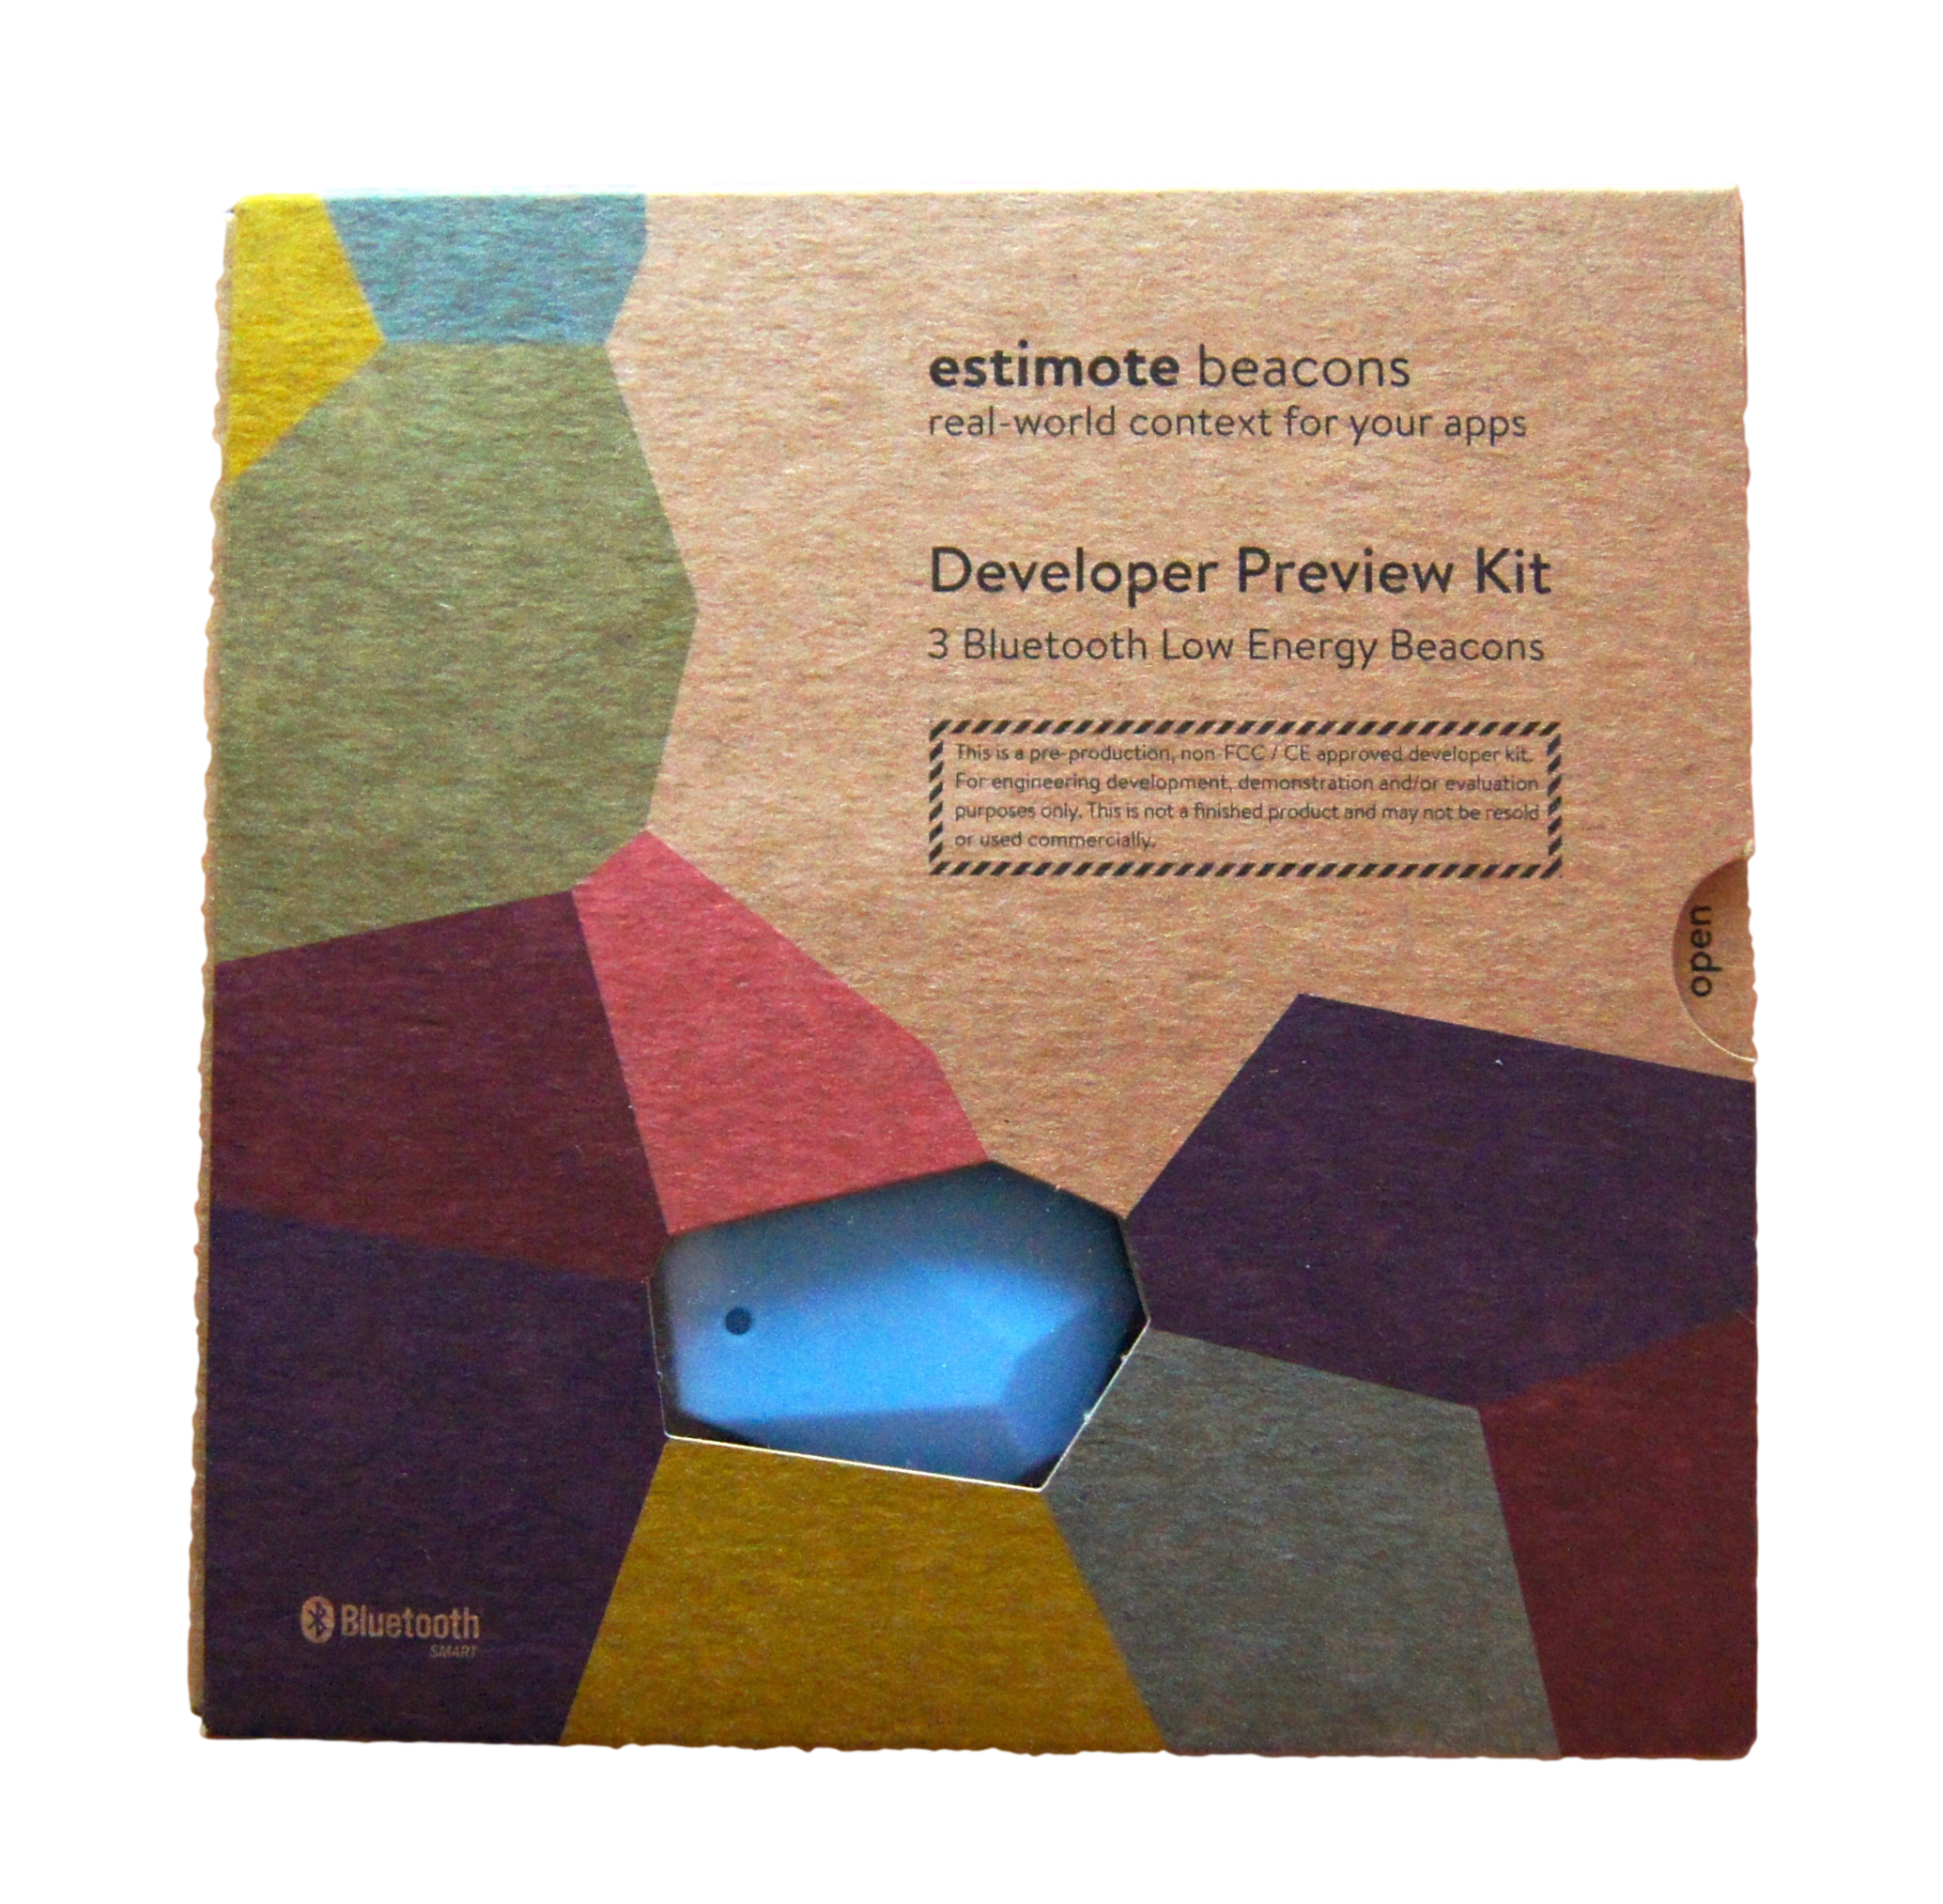
\includegraphics[scale=0.1]{estimote-developer-kit}
	\caption{Das Developer-Kit von estimote}
	\label{estimote-developer-kit}
\end{figure}

Im inneren des Beacons befindet sich ein Bluetooth Chipsatz von Nordic Semiconductor, welcher auf einem 32-bit ARM Prozessor beruht und mit einem 2,4Ghz Bluetooth Low Energy Modul arbeitet. Dabei verfügt der über 256 KB Flash-Speicher für Speicherung der Beacon-Konfiguration.
Speziell in den estimote-Beacon wurde dazu noch ein Temperatursensor eingebaut, welcher allerdings momentan noch nicht angesprochen werden kann.

Des Weiteren stellt estimote noch ein SDK für Android und iOS zur Verfügung, welches in Fall des iOS-SDK auf der iBeacons-API basiert, jedoch speziell auf die estimote-Beacons abgestimmt ist. 
Dabei bietet es neben den Funktionen der iBeacon-API noch die Funktionalität, sich mit den estimote Beacons zu verbinden und diese zu programmieren. So erlaubt es zum Beispiel die Signalstärke, das Sendeintervall und die Major-Minor-Informationen zu verändern oder die Firmware der Beacons zu aktualisieren.

Da das SDK, bis auf die Programmierung der Beacons, keine Vorteile gegenüber dem Core Location-Framework mit der iBeacons-API bietet, wurde jedoch auf die Verwendung verzichtet.

%%%%%%%%%%%%%%%%%%%%%%%%%%%%%%%%%%%%%%%%%%%%%%%%%%%%%%%%%%%%
\subsection{kontakt.io Beacon}
\label{sec:dataandmeasurement:mobilebeacon:kontaktio}
%%%%%%%%%%%%%%%%%%%%%%%%%%%%%%%%%%%%%%%%%%%%%%%%%%%%%%%%%%%%
Ein weiteres Unternehmen, welches sich eine eigene iBeacons-Lösung anbietet ist \emph{kontakt.io}. Auch hier ist noch kein finales Produkt erhältlich, sondern nur ein \emph{Development Kit}, welches zehn Beacons enthält. 
Die Beacons sind relativ schlicht gehalten und das Innere ist sehr einfach zugänglich, sodass ein Batteriewechsel ohne Umstände möglich ist.


\begin{figure}[htb!]
		\centering
	\includegraphics[scale=0.1]{kontakt-beacon-outside}
	\caption{Kontakt.io Beacon}
	\label{kontakt-beacon-outside}
\end{figure}

Die Beacons von \emph{kontakt.io} basieren dabei auf dem BLE113 Chipsatz von \emph{bluegiga}, welcher über 256 KB Flash-Speicher verfügt und einen 8051 Mikrocontroller von Intel nutzt.


Auch kontakt.io bietet ein eigenes SDK an, welches im Gegensatz zu dem SDK von \emph{estimote} nicht nativ für die einzelnen Plattformen entworfen wurde, sondern online über eine REST-Schnittstelle arbeitet.
Dabei stellt \emph{kontakt.io} ein Webpanel zur Verfügung, in welchem man die einzelnen Beacons mit ihrem UUID, Major und Minor-Wert registriert und jedem den jeweiligen Ort beziehungsweise die Funktion zuweisen kann. 
Auch auf die Verwendung dieses SDK wurde verzichtet.


%%%%%%%%%%%%%%%%%%%%%%%%%%%%%%%%%%%%%%%%%%%%%%%%%%%%%%%%%%%%
\section{Stationäre iBeacons}
\label{sec:dataandmeasurement:stationarybeacon}
%%%%%%%%%%%%%%%%%%%%%%%%%%%%%%%%%%%%%%%%%%%%%%%%%%%%%%%%%%%%
Neben den mobilen iBeacons, welche mittels Batterien betrieben werden, gibt es auch stationäre iBeacons, welche auf eine stetige Anbindung an das Stromnetz angewiesen sind.
Dabei gibt es verschiedene Ansätze.
Zum Einen bieten zum Beispiel \emph{PayPal} und \emph{Radius Networks} einen Ansatz, bei dem die komplette Technik in einen USB-Stick integriert wird und über ein USB-Netzteil an jeder Steckdose betrieben werden kann. Die verwendete Technik dieser Beacons entspricht denen der batteriebetriebenen Beacons.

Eine andere Lösung ist die Nutzung eines Bluetooth 4.0-kompatiblen USB-Dongles an einem Computer. Dieser kann mit entsprechender Software zu einem iBeacon umfunktioniert werden.

%%%%%%%%%%%%%%%%%%%%%%%%%%%%%%%%%%%%%%%%%%%%%%%%%%%%%%%%%%%%
\subsection{Raspberry Pi als iBeacon}
\label{sec:dataandmeasurement:stationarybeacon:raspberrypi}
%%%%%%%%%%%%%%%%%%%%%%%%%%%%%%%%%%%%%%%%%%%%%%%%%%%%%%%%%%%%
Der Raspberry Pi ist ein Mini-Computer, welcher auf einem ARM-Prozessor basiert und als günstiger Computer für Programmiereinsteiger konzipiert wurde. Der kleine Computer ermöglicht aber auch andere Einsatzgebiete, zum Beispiel als Beacon.

Um den Raspberry Pi zu einem Beacon umzufunktionieren wurde eine Linux-Distribution auf dem Gerät installiert und ein Bluetooth-Dongle über USB angeschlossen. Dabei kam ein Modul von \emph{Plugable Technologies} zum Einsatz, welches spezielle Bluetooth 4.0 und Linux-Unterstützung bietet.
Für die Umfunktionierung zum iBeacon wurde die Bluetooth-Implementierung \emph{blueZ} eingesetzt, welche es erlaubt das Bluetooth-Modul anzusprechen und spezifische Nachrichten über Bluetooth zu versenden.
Diese Möglichkeit den Raspberry Pi als iBeacon zu nutzen, wurde von der Firma Radius Network vorgestellt. Diese bieten ein ausführliches Tutorial für die Nutzung des Raspberry Pi als iBeacon auf ihrer Webseite an (\citet{radiusraspberry}), welches von mir genutzt wurde, um den Raspberry Pi zu konfigurieren.

%%%%%%%%%%%%%%%%%%%%%%%%%%%%%%%%%%%%%%%%%%%%%%%%%%%%%%%%%%%%
\section{Physikalische Grundlagen}
\label{sec:dataandmeasurement:physics}
%%%%%%%%%%%%%%%%%%%%%%%%%%%%%%%%%%%%%%%%%%%%%%%%%%%%%%%%%%%%
Im Vergleich zu Kabelverbindungen, wo die Ausbreitung des Signals entlang eines bestimmten Leiters geschieht, ist die Ausbreitung eines drahtlosen Signals von deutlich mehr Faktoren abhängig.

\textbf{Dämpfung}

Dämpfung ist die Schwächung der Energie, mit welcher das Signal übertragen wird. Diese tritt auch bei einer freien Sichtverbindung zwischen Sender und Empfänger auf. Die Verringerung der Leistung ist dabei abhängig von der Ausgangssendeleistung $P_0$ und der Entfernung $r$ zwischen Sender und Empfänger. Die letztlich am Empfänger ankommende Signalstärke $P_r$ berechnet sich dabei wie folgt:

\begin{equation}
	P_r = \frac{P_0}{r^{2}} 
\end{equation}

Die Abschwächung des Signals resultiert aus der Art der Aussendung. Da die hier verwendeten Beacons einem Punktstrahler entsprechen, wird die anliegende Signalstärke auf eine Kugeloberfläche verteilt. Die Kugeloberfläche $O$ lässt sich dabei abhängig vom Radius $r$ mittels der Formel $O = 4 \pi r^{2}$ berechnen. Die Oberfläche vergrößert sich damit quadratisch zum Radius.

\textbf{Abschattung}

Die Abschattung ist eine stärkere Form der Dämpfung, welche durch Objekte zwischen der Signalquelle und dem Empfänger verursacht wird. Die Abschattung ist dabei abhängig von der Frequenz des Signals und der Geschaffenheit des Objektes. Bei höherer Frequenz ist eine stärkere Abschattung des Signals gegeben.

\textbf{Reflexion}

An größeren Oberflächen kann es zu Reflexionen des Signals kommen. Dabei trifft es auf die Oberfläche und wird dann in abgeschwächter Form reflektiert.

\textbf{Streuung}

Ähnlich der Reflexion trifft das Signal auf eine Oberfläche, wird dabei jedoch aufgespalten und in verschiedene Richtung abgelenkt.

\textbf{Mehrwegeausbreitung}

Durch die obene genannten Effekte ist es möglich, das ein Signal einen Empfänger auf mehreren Wegen erreicht. Dabei ist die Signalstärke stark abhängig von dem zurückgelegtem Weg. Ausserdem unterscheiden sich die Laufzeiten der Signale, da diese ebenfalls vom Weg abhängig sind. Dadurch kann es auch zu Überlagerungen zwischen Signalen kommen, welche zur gleichen Zeit gesendet wurden, jedoch zu unterschiedelichen Zeiten beim Empfänger eintreffen. 
Durch diese Phasenverschiebung kann das Signal zusätzlich abgeschwächt werden.


%%%%%%%%%%%%%%%%%%%%%%%%%%%%%%%%%%%%%%%%%%%%%%%%%%%%%%%%%%%%
\section{Außenmessungen}
\label{sec:dataandmeasurement:outdoormeasure}
%%%%%%%%%%%%%%%%%%%%%%%%%%%%%%%%%%%%%%%%%%%%%%%%%%%%%%%%%%%%

%%%%%%%%%%%%%%%%%%%%%%%%%%%%%%%%%%%%%%%%%%%%%%%%%%%%%%%%%%%%
\section{Innenraummessungen}
\label{sec:dataandmeasurement:indoormeasure}
%%%%%%%%%%%%%%%%%%%%%%%%%%%%%%%%%%%%%%%%%%%%%%%%%%%%%%%%%%%%
Um die Leistungsfähigkeit und das Verhalten der Beacons in Innenräume zu testen und darzustellen, wurden verschiedene Messungen durchgeführt. Dazu wurden zum einen die mobilen Beacons verwendet und zum Anderen der Raspberry Pi, als stationäres Beacon.
Die Messungen wurden dabei sowohl mit dem iPhone 5 als auch mit dem iPhone 4s durchführt, um auch hier die Unterschiede zwischen den einzelnen Modellen zu erfassen.


Zuerst wurden die Messungen mit den mobilen Beacons, hier die \emph{kontakt.io}-Beacons, durchgeführt.
Diese wurden in einem leeren, nur an den Wänden bestellten, Raum durchgeführt, wobei immer freie Sicht zwischen den Beacons und den Empfangsgeräten bestand. Für jede Entfernung wurden dabei 100 Stichproben genommen, jeweils eine pro Sekunde.
%%%%%%%%%%%%%%%%%%%%%%%%%%%%%%%%%%%%%%%%%%%%%%%%%%%%%%%%%%%%
% figure of signal strnegth
%%%%%%%%%%%%%%%%%%%%%%%%%%%%%%%%%%%%%%%%%%%%%%%%%%%%%%%%%%%%
\begin{figure}[h!]
	\centering
	\begin{minipage}[t]{5cm}
		\includegraphics[scale=0.2]{avgiphone5}
		\caption{Messung des iPhone 5}
		\label{avgiphone5-signalstrength}
	\end{minipage}
	\hspace{2cm}
	\begin{minipage}[t]{5cm}
			\includegraphics[scale=0.2]{avgiphone4s}
			\caption{Messung des iPhone 4s}
			\label{avgiphone4s-signalstrength}
	\end{minipage}
		\caption{Durchschnittliche Signalstärke eines kontakt.io Beacons}
		\label{signalstrength}
\end{figure}

In Abbildung \ref{avgiphone5-signalstrength} und Abbildung \ref{avgiphone4s-signalstrength} lässt sich dabei sehr gut erkennen, das die Signalstärke, nicht wie eigentlich erwartet stetig abnimmt, sondern relativ stark schwankt. Dies ist darauf zurückzuführen, dass in Innenräumen sowohl Wände, als auch Gegenstände im Raum, das Bluetooth-Signal reflektieren oder blockieren und so die Ergebnisse verfälschen.
Des Weiteren ist zu erkennen, dass die Ergebnisse zwischen den verschiedenen iPhone-Modellen deutlich voneinander abweichen. Das lässt darauf schließen, das der verbaute Chipsatz beziehungsweise die verbaute Antenne innerhalb der Gerät die Ergebnisse deutlich beeinflusst und die Werte daher nur schwer übertragbar sind.

Ein weiterer wichtiger Punkt ist die Untersuchung der Stabilität des Signal. Dabei wurden die gleichen Daten wie zuvor verwendet, jedoch um die minimalen und maximalen Werte ergänzt. In Abbildung \ref{all-iphone5} lässt sich dabei gut erkennen, das die Ergebnisse eine ähnliche Tendenz haben, aber sich dennoch über einen sehr großen Bereich der Signalstärke verteilen.

\begin{figure}[htb!]
		\centering
	\includegraphics[scale=0.5]{alliphone5}
	\caption{Minimale, maximale und durchschnittliche Signalstärke des Beacons gemessen vom iPhone 5}
	\label{all-iphone5}
\end{figure}


Zusätzlich wurde untersucht in wie weit sich die Sendeleistung und Signalqualität der batteriebetriebenen Beacon von stationären Beacons unterscheidet.
Dazu wurde der gleiche Messaufbau wie zuvor genutzt, jedoch das \emph{kontakt.io} Beacon durch den Raspberry Pi ausgetauscht. Danach wurden die gleichen Messungen erneut durchgeführt.

\begin{figure}[htb!]
		\centering
	\includegraphics[scale=0.5]{avgiphone5_raspberry}
	\caption{Durchschnittliche Signalsteäines Raspberry Pi Beacons}
		\label{avgiphone5_raspberry}
\end{figure}

Wie aus Abbildung \ref{avgiphone5_raspberry} zu entnehmen, sind die Ergebnisse im Vergleich zu der Messung der kontakt.io Beacons näher am erwarteten Ergebnis, welches eine konstante Abnahme der Signalstärke sein sollte. Es sind jedoch immernoch einige Ausreißer zu erkennen. Bei der Betrachtung der minimalen und maximalen Signalstärken fällt auch auf, dass die ähnlich stark schwanken, wie schon zuvor bei den kontakt.io Beacons. Die Stabilität des Signal des stationären Beacons ist also genauso schwach beziehungsweise noch schwächer als die des batteriebetriebenen Beacons. Dies wird in Abbildung \ref{alliphone5_raspberry} nocheinmal deutlich.

\begin{figure}[htb!]
		\centering
	\includegraphics[scale=0.5]{alliphone5_raspberry}
	\caption{Minimale, maximale und durchschnittliche Signalstrke des Raspberry Pi gemessen vom iPhone 5}
	\label{alliphone5_raspberry}
\end{figure}

Für die weiteren Test und Messungen wurden daher die \emph{kontakt.io} Beacons verwendet, da die beiden zur Verfügung stehenden Beacons sich in Signalstärke und Stabilität nicht zu stark unterscheiden, von den \emph{kontakt.io} Beacons jedoch deutlich mehr Exemplare verfügbar sind und diese deutlich variabler im Bezug auf die Positionierung der Beacons sind.


%%%%%%%%%%%%%%%%%%%%%%%%%%%%%%%%%%%%%%%%%%%%%%%%%%%%%%%%%%%%
\section{Mögliche Störfaktoren}
\label{sec:dataandmeasurement:interferencefactor}
%%%%%%%%%%%%%%%%%%%%%%%%%%%%%%%%%%%%%%%%%%%%%%%%%%%%%%%%%%%%
Wie die obigen Messungen zeigen, weichen die realen Ergebnisse stark von den, durch die physikalischen Ausbreitungseigenschaften der elektromagnetischen Wellen, angenommenen Ergebnissen ab. Dies hängt vorallem damit zusammen, dass die Antenne der Beacons nicht gerichtet ist, sondern in alle Richtungen sendet. Dies führt dazu, dass das Signal der Beacons von diversen Flächen im Raum reflektiert und so nicht auf direktem Weg zum Endgerät gelangt. 

Ein weiterer wichtiger Störfaktor ist der Benutzer selbst, da der menschliche Körper größtenteils aus Wasser besteht, welche elektromagnetische Wellen abschirmt. Daher ist zu beobachten, dass die Ausrichtung des Nutzers einen deutlichen Einfluss auf die Signalstärke nimmt. In Abbildung \ref{boxplotiPhone5Body} ist diese Auswirkung des Körpers deutlich zu erkennen. Hierbei wurden jeweils aus zwei Metern Entfernung 100 Stichproben der Signalstärke genommen. Einmal mit freier Sicht zum Beacon und einmal mit dem Körper zwischen Beacon und iPhone. 

\begin{figure}[htb!]
		\centering
	\includegraphics[scale=0.5]{boxplotiPhone5Body}
	\caption{Signalstärke bei 2m Entfernung zum Beacon}
	\label{boxplotiPhone5Body}
\end{figure}

Auf der Abbildung ist deutlich zu erkennen wie der Körper die Signalstärke verringert. Dieser Faktor muss also in die Positionsbestimmung einbezogen werden.

Zusätzlich zum Körper kann es an realen Einsatzorten weitere Gegenstände geben, welche das Signal abschirmen beziehungsweise abschwächen, wie zum Beispiel Wände oder Möbelstücke.
\chapter{Umsetzung und Implementation}
\label{chap:implementation}

%%%%%%%%%%%%%%%%%%%%%%%%%%%%%%%%%%%%%%%%%%%%%%%%%%%%%%%%%%%%
\section{Ansatz zur Positionsbestimmung}
\label{sec:implementation:positioning}
%%%%%%%%%%%%%%%%%%%%%%%%%%%%%%%%%%%%%%%%%%%%%%%%%%%%%%%%%%%% 
Bei der Positionsbestimmung geht es um die Bestimmung des aktuellen Ortes in Echtzeit und das auf bis zu wenige Meter genau. Bei der Positionsangabe handelt es sich hier um eine zweidimensionale Position, da dies für die Indoor-Positionierung ausreichend ist.

Bei der Positionsbestimmung wurden zwei verschiedene Ansätze untersucht. Zum einen die Trilateration, welche eine Positionierung mittels Entfernungen zu verschiedenen Fixpunkten ermöglicht und zum anderen die Positionierung mittels Fingerprinting, welches eine Datenbank mit sogenannten Fingerprints, also vorher aufgezeichneten Messwerten und damit verbundenen Positionsdaten, voraussetzt und über diese Daten die aktuelle Position bestimmt.

Die Positionsbestimmung soll dabei in einem 2D-Raum erfolgen, da die Höhe vernachlässigt werden kann. In der realen Welt kann die Höhe ebenfalls vernachlässigt werden, da dort Stockwerke meist einen deutlichen Höhenunterschied aufweisen, sodass dieser über andere Faktoren eindeutig bestimmt werden kann.

%%%%%%%%%%%%%%%%%%%%%%%%%%%%%%%%%%%%%%%%%%%%%%%%%%%%%%%%%%%%
\subsection{Trilateration}
\label{sec:implementation:trilateration}
%%%%%%%%%%%%%%%%%%%%%%%%%%%%%%%%%%%%%%%%%%%%%%%%%%%%%%%%%%%%
Die Trilateration ist eine Methode zur Bestimmung der aktuellen Position. Im Gegensatz zur Triangulation, welche die Position anhand der Winkelgrößen zwischen verschiedenen Fixpunkten bestimmt, wird bei der Trilateration die Position durch die Abstände zu den Fixpunkten bestimmt. 

Die Trilateration macht sich dabei zunutze, dass sich ein Objekt, bei gegebenem Abstand zum Fixpunkt, auf einer Kreisbahn um diesen befinden muss. Der Radius des Kreises entspricht dabei dem Abstand. Für eine genaue Positionierung sind dabei mindestens drei Fixpunkte und deren Abstände nötig, da nur so ein eindeutiger Schnittpunkt bestimmt werden kann. \cite{wlanposlateration}.

\begin{figure}[htb!]
	\centering
	\includegraphics[scale=1.5]{trilateration}
	\caption{Funktionsprinzip der Trilateration}
	\label{trilateration-accurate}
\end{figure}

In Abbildung \ref{trilateration-accurate} sieht man dabei die Funktionsweise der Trilateration bei genauer Abstandsbestimmung. Dabei entsteht ein eindeutiger Schnittpunkt aller Kreise. In realen Messungen und Positionsbestimmungen ist es jedoch nicht möglich die exakten Abstände zu bestimmen, da es immer zu Messungenauigkeiten kommen kann.
Bei solchen ungenauen Messungen ist es nun nicht mehr möglich einen genauen Schnittpunkt zu definieren. 

Um diese Ungenauigkeit auszugleichen wird das Verfahren entsprechend angepasst. Dabei werden Geraden durch die Schnittpunkte der einzelnen Umkreise gelegt. Dadurch entsteht zwischen den Geraden ein neuer Schnittpunkt, welcher die aktuelle Position repräsentiert. Dieses Verfahren wird in Abbildung \ref{trilateration-inaccurate} dargestellt.

\begin{figure}[htb!]
		\centering
	\includegraphics[scale=1.5]{trilateration-inaccurate}
	\caption{Trilateration bei ungenauen Abständen zu den Fixpunkten}
	\label{trilateration-inaccurate}
\end{figure}

Damit ist es möglich auftretende Ungenauigkeiten zu kompensieren und trotzdem eine genaue Positionsbestimmung durchzuführen.

Bei der genutzten iBeacons beziehungsweise Bluetooth-Technologie ist eine genaue Entfernungsangabe jedoch nicht vorgesehen, wodurch das Verfahren der Trilateration nicht direkt angewandt werden kann. Dafür muss zunächst ein Ersatzindikator für die Entfernungsmessung bestimmt werden.
Bei der Bluetooth-Technologie bietet sich dafür die Signalstärke an.
Dabei wird die Tatsache genutzt, dass die Signalstärke mit zunehmendem Abstand sinkt und man somit aus der aktuellen Signalstärke auch die aktuelle Entfernung bestimmen kann. 
Das Verhältnis zwischen Entfernung und Signalstärke bei elektromagnetischen Wellen wird durch das Abstandsgesetz beschrieben, welches besagt, das die Signalstärke quadratisch zum Abstand abnimmt.

\begin{equation}
	\text{\emph{Signalstärke}} = \frac{\text{\emph{Ausgangssignalstärke}}}{\text{\emph{Entfernung}}^2}
\end{equation}

Diese Annahme mag bei freien Flächen korrekt sein, in Innenräumen kommen jedoch weitere Faktoren hinzu, wie in Kapitel \ref{sec:dataandmeasurement:interferencefactor} beschrieben. 
Durch Wände und Hindernisse im Raum, wie zum Beispiel Schränke, Regale, usw., kommt es dort zu einer Dämpfung des Signals, wodurch die Signalstärke beeinflusst wird. Des Weiteren kann es in Innenräumen auch zu Streuung und Reflexionen kommen, welche das Signal zusätzlich verfälschen.

Diese Annahme bestätigt sich auch bei den Messungen in Kapitel \ref{chap:dataandmeasure}. Diese zeigen, dass die gemessene Signalstärke nicht, wie angenommen, mit der Entfernung stetig abnimmt, sondern sehr stark schwankt, wodurch keine genaue Entfernungsbestimmung durchgeführt werden kann.

Die Methode der Trilateration wurde auf Grund der fehlenden Genauigkeit verworfen. 

%%%%%%%%%%%%%%%%%%%%%%%%%%%%%%%%%%%%%%%%%%%%%%%%%%%%%%%%%%%%
\subsection{Fingerprinting}
\label{sec:implementation:positioning:fingerprinting}
%%%%%%%%%%%%%%%%%%%%%%%%%%%%%%%%%%%%%%%%%%%%%%%%%%%%%%%%%%%%
Das Fingerprinting ist ein Verfahren zur Positionierung auf der Grundlage von gesammelten Signalstärke-Werten.

Für das Fingerprinting werden dabei für verschiedene Positionen im untersuchten Messraum die Signalstärken der vorhandenen Bluetooth-Signale aufgezeichnet. 
Dadurch entsteht ein charakteristischer Fingerabdruck der Signalstärken an der aktuellen Position \cite{wififingerprinting}.

Bei der Positionierung wird daraufhin der aktuelle Fingerabdruck mit den zuvor aufgezeichneten Abdrücken verglichen, wodurch die aktuelle Position bestimmt werden kann.

Dieses Verfahren ist vor allem für die Positionierung mittels Signalstärken gedacht, da die möglichen Störungen des Signals bereits bei der Aufzeichnung der Fingerprints berücksichtigt werden.

Das Fingerprinting-Verfahren besteht aus zwei Phasen.


\textbf{Vorbereitungen}

Um eine Positionierung mittels Fingerprinting zu erlauben, muss der Messraum, in welchem die Positionierung stattfindet, zunächst in ein Gitternetz unterteilt werden. Dabei repräsentiert jede Zelle dieses Gitternetzes eine mögliche Position im Raum.
Die Größe dieser Zellen ist prinzipiell frei wählbar, wird jedoch im Wesentlichen durch zwei Faktoren bestimmt. 

Zum einen hängt die Zellengröße von der gewünschten Genauigkeit ab, da jede Zelle eine mögliche Position repräsentiert. Folglich erhöht eine kleinere Zellengröße die Genauigkeit der Positionierung.

Der zweite Faktor bei der Wahl der Zellengröße, ist die Eindeutigkeit einer Zelle. Dies ist darauf zurückzuführen, dass bei kleineren Zellen die Differenzen der Messwerte zwischen den einzelnen Zellen abnehmen.
Es ist daher nötig die Zelle ausreichend groß zu wählen, sodass eine gute Unterscheidung zwischen einzelnen Zellen möglich ist.

Aufgrund dieser zwei Kriterien muss die Zellengröße so gewählt werden, dass eine akzeptable Genauigkeit gegeben ist und eine eindeutige Unterscheidung der Zellen möglich ist.


\textbf{Trainingsphase}


Die erste Phase ist die sogenannte \emph{Trainingsphase} (auch Offlinephase). Dabei werden die Fingerprints gesammelt, welche letztlich zur Positionsbestimmung genutzt werden.

Ein Fingerprint besteht dabei aus einem Zeitstempel, der aktuellen Position und den Signalstärken der Sendestationen, in diesem Fall der Beacons, welche sich aktuell in Reichweite befinden.

In der Trainingsphase werden dabei für jede Zelle eine Reihe von Fingerprints gesammelt. Die Anzahl der zu sammelnden Fingerprints sollte dabei ausreichend groß sein, sodass Messfehler kompensiert werden können.

Da in der Trainingsphase eine Reihe von Fingerprints für jede vorhandene Zelle erhoben werden müssen, ist die Trainingsphase relativ aufwendig.


\textbf{Onlinephase}


In der zweiten Phase, auch \emph{Onlinephase} genannt, werden die zuvor gesammelten Informationen verwendet um die aktuelle Position zu bestimmen. 

Dafür werden die gesammelten Fingerprints mit den aktuell gemessenen Signalstärken abgeglichen. Für die Positionierung kann dabei auf verschiedene Algorithmen zurückgegriffen werden.

Es wurden hier drei verschiedene Algorithmen untersucht. Die ersten beiden Algorithmen basieren auf dem Nearest-Neighbor-Verfahren. Dabei werden im ersten Algorithmus alle gesammelten Fingerprints mit dem aktuell gemessenen Fingerprint verglichen. Der zweite Algorithmus arbeitet ähnlich, nutzt jedoch die Mittelwerte der jeweiligen Signalstärken in einer Zelle. 
Der letzte Algorithmus arbeitet über eine Wahrscheinlichkeitsverteilung der Signalstärken.


Durch die Vorteile des Fingerprintings bei der Positionierung mittels Signalstärken und der Robustheit des Verfahrens gegenüber Signalverfälschungen durch statische Objekte wurde dieses Verfahren für die Realisierung der Indoor Positionierung ausgewählt.


%%%%%%%%%%%%%%%%%%%%%%%%%%%%%%%%%%%%%%%%%%%%%%%%%%%%%%%%%%%%
\section{Erstellung der iOS-Applikation}
\label{sec:implementation:iosapplication}
%%%%%%%%%%%%%%%%%%%%%%%%%%%%%%%%%%%%%%%%%%%%%%%%%%%%%%%%%%%%

Die geplante iOS-Applikation soll alle Bereiche des Fingerprintings abdecken. 
Das heißt, sie soll sowohl die Sammlung von Fingerprints an bestimmten Orten ermöglichen, als auch die Lokalisierung des Gerätes innerhalb des Messraumes erlauben.
Außerdem soll eine Ausgabe der gesammelten Daten ermöglicht werden, sodass man in der App zum Beispiel die Anzahl der gesammelten Fingerprints für jede Zelle auslesen kann.
Um dies zu erreichen, muss die iOS-Applikation über mehrere Views verfügen, welche jeweils eine dieser Aufgaben erfüllen.

Für die Navigation zwischen den einzelnen Views kommt dafür ein TabBarController zum Einsatz. Dieser ermöglicht es, mittels einer Leiste am unteren Bildschirmrand, zwischen verschiedenen Views zu wechseln.


%%%%%%%%%%%%%%%%%%%%%%%%%%%%%%%%%%%%%%%%%%%%%%%%%%%%%%%%%%%%
\subsection{Initialisierung des Projektes}
\label{sec:implementation:iosapplication:initializing}
%%%%%%%%%%%%%%%%%%%%%%%%%%%%%%%%%%%%%%%%%%%%%%%%%%%%%%%%%%%%

Für die Implementierung der iOS-Applikation muss zunächst ein neues Projekt in Xcode erstellt werden. Wie bereits in Kapitel \ref{sec:tools:xcode} erwähnt, gibt es dabei verschiedene Vorlagen, aus welchen gewählt werden kann. Für diese Applikation wurde deshalb die Vorlage der \emph{Master-Detail Application} mit CoreData-Unterstützung gewählt. Dies erzeugt automatisch ein CoreData-Modell und alle erforderlichen Objekte, um dieses zu nutzen. Außerdem werden noch weitere Dateien generiert, wie etwa das Storyboard und die AppDelegate.
Das Storyboard beinhaltet bereits einen Master-Detail-View, lässt sich jedoch beliebig erweitern und bearbeiten. 

\begin{figure}[htb!]
		\centering
	\includegraphics[scale=0.25]{ipad-master-detail-view-controller-mockup}
	\caption{Beispiel einer Master-Detail Applikation auf dem iPad}
	\label{master-detail-view-controller}
\end{figure}

Die AppDelegate ist die Kerndatei der Applikation und steuert dabei das Verhalten bei Start und bei Beendigung der Applikation. So werden dort bei Start der Applikation die nötigen Objekte für den Zugriff auf die CoreData-Funktionalitäten erzeugt und an die jeweiligen ViewController der Applikation weitergegeben.


%%%%%%%%%%%%%%%%%%%%%%%%%%%%%%%%%%%%%%%%%%%%%%%%%%%%%%%%%%%%
\subsection{Erstellung der Oberfläche}
\label{sec:}
%%%%%%%%%%%%%%%%%%%%%%%%%%%%%%%%%%%%%%%%%%%%%%%%%%%%%%%%%%%%

Mittels des Interface Builders wird die Oberfläche der Applikation angepasst. Dazu wird die Storyboard-Datei für das iPhone editiert.
Durch die Nutzung der Master-Detail-Application Vorlage beinhaltet das Storyboard bereits zwei Views, welche in einen Navigation Controller eingebettet sind. 
Zum einen den Master View, welcher aus einer Tabelle besteht und dem Detail View, welcher bei Klick auf eine Tabellenzeile weitere Informationen über diese ausgibt. 
Der Navigation Controller steuert dabei die Übergänge zwischen den beiden Views.
Diese Views werden in dieser Applikation behalten und später für die Anzeige der bereits gesammelten Fingerprint-Informationen genutzt.

Als erstes wird ein TabBarController zum Storyboard hinzugefügt. Dieser besitzt bei der Erzeugung bereits zwei Tabs mit jeweils einem leeren View. Diese beiden Views werden später für die Sammlung der Fingerprints und die Positionierung verwendet.

Der bereits vorhandene Master-View wird in den TabBarController integriert, sodass dieser nun aus drei Tabs besteht. Außerdem werden die beiden leeren Views in einen NavigationController eingebettet.

\begin{figure}[htb!]
		\centering
	\includegraphics[scale=0.25]{iphone-tab-view-controller-mockup}
	\caption{Beispiel eines TabView Controller auf dem iPhone 5}
	\label{iphone-tab-view-controller}
\end{figure}

Nachdem das grundlegende Layout erstellt wurde, werden die einzelnen Views konfiguriert.

\textbf{FingerprintingSetupView}


Der \emph{FingerprintingSetupView} wird genutzt, um die aktuelle Zelle für die Sammlung der Fingerprints zu konfigurieren und um die gewünschte Anzahl von Fingerprints einzustellen. Da die Applikation nur zu Testzwecken eingesetzt werden soll, wird die Erscheinung des View sehr simpel gehalten. 
Der View besteht dabei lediglich aus zwei Textfeldern und mehreren Button. 
Ein Textfeld erlaubt die Eingabe der aktuellen Zelle und das andere die Anzahl der zu sammelnden Fingerprints.
Außerdem befinden sich unter jedem Feld zwei Buttons, welche es erlauben, die Werte innerhalb der Felder zu inkrementieren oder zu dekrementieren.

Zusätzlich befindet sich in dem View ein weiterer Button, welcher es erlaubt die Sammlung der Fingerprints zu starten. 
Nach dem Start wird dabei der FingerprintingView aufgerufen.


\textbf{FingerprintingView}

Der \emph{FingerprintingView} ist ebenfalls sehr simpel aufgebaut.
Er besteht aus einem Label, welches die Anzahl der aktuell gefundenen Beacons anzeigt.
Außerdem zeigt er den aktuellen Forschritt des Sammelvorganges an. Dafür dient zum Einen ein Progress View, welcher mittels einer Statuslinie den aktuellen Vortschritt anzeigt. Zum Anderen liegt darunter ein Label, welches den aktuellen Fortschritt in Prozent anzeigt.

In der NavigationBar des NavigationController existiert außerdem ein Button, welcher es erlaubt das Sammeln der Fingerprints direkt abzubrechen und damit zum vorherigen View zurückzukehren. Nach Abschluss des Sammelvorgangs soll die Applikation automatisch zum vorherigen View zurückkehren.


\textbf{PositioningView}

Der \emph{PositioningView} besteht aus Labels, welche die aktuelle Zelle anzeigen. Dabei wird die aktuelle Position für jeden implementierten Algorithmus ausgegeben, sodass sich diese Ergebnisse direkt vergleichen lassen. Außerdem befindet sich im unteren Bereich des PositioningViews eine MapView, welcher die Karte des aktuellen Raumes ausgeben soll.


\textbf{InformationView} 
Der InformationView basiert auf dem MasterView, welcher durch die Nutzung des Templates automatisch generiert wurde. Daher besteht dieser bereits aus einem TableView.
Dieser soll dabei die Zellen anzeigen, für welche bereits Fingerprints gesammelt wurden. Bei einem Klick auf eine Zelle wird dabei der InformationDetailView aufgerufen.

\textbf{InformationDetailView}
Der InformationDetailView zeigt detailierte Informationen der Zelle an, wie etwa die Anzahl der gesammelten Fingerprints oder die durchschnittliche Signalstärke der Beacons.
Diese werden in einer Tabellenansicht dargestellt.


%%%%%%%%%%%%%%%%%%%%%%%%%%%%%%%%%%%%%%%%%%%%%%%%%%%%%%%%%%%%
\subsection{Erstellung des CoreData-Modells}
\label{sec:}
%%%%%%%%%%%%%%%%%%%%%%%%%%%%%%%%%%%%%%%%%%%%%%%%%%%%%%%%%%%%
Für die Speicherung der Fingerprints wird das CoreData-Framework verwendet. Dafür wurde bei der Erstellung des Projektes ein Modelldatei erzeugt. In dieser lässt sich der Aufbau des Projektes erstellen und bearbeiten.
Zuerst müssen verschiedene Entitäten erstellt werden, welche die Daten im Speicher repräsentieren.
Für die grundlegende Sammlung von Fingerprints benötigt man vier Entitäten: Cell, Beacon, Fingerprint und Measurement.

Für eine schnellere Durchführung des zweiten Algorithmus, welcher mit den Mittelwerten der Beacons in einer Zelle arbeitet, wird eine weitere Entität angelegt. Die \emph{BeaconInCell}-Entität repräsentiert dabei ein Beacon in einer Zelle.
Um den dritten Algorithmus zu ermöglichen, ist noch eine zusätzliche Entität nötig. Die \emph{BeaconInCellProbabilty}-Entität verwaltet dabei die Wahrscheinlichkeitsverteilung eines Beacons in einer Zelle.

Im Folgenden werden die einzelnen Entitäten genauer erklärt.


\textbf{Cell}

Repräsentiert eine Zelle des Messraumes. Besitzt als Attribut die Zellennummer.
Diese besitzt eine \emph{One-to-many}-Beziehung zu BeaconInCell und Fingerprints.


\textbf{BeaconInCell}

Repräsentiert ein Beacon in einer bestimmten Zelle. Besitzt als Attribute sowohl die durchschnittlichen, maximale und minimale Signalstärke als auch deren Median.
Außerdem existiert eine \emph{One-to-many}-Beziehung zu Measurements und BeaconInCellProbabilty.



\textbf{BeaconInCellProbability}

Repräsentiert den Wahrscheinlichkeitswert für eine Signalstärke eines Beacons in einer Zelle.
Daher besitzt es als Attribute die Wahrscheinlichkeit und die Signalstärke.

\textbf{Beacon}

Repräsentiert ein Beacon und beinhaltet als Attribute die UUID, den Major-Wert und den Minor-Wert des Beacons.
Außerdem besitzt die Entität eine \emph{One-to-many}-Beziehung zu BeaconInCell.

\textbf{Fingerprint}

Repräsentiert einen Fingerprint und beinhaltet als Attribut einen Zeitstempel.
Die Entität verfügt darüberhinaus über eine \emph{One-to-many}-Beziehung zu Measurements.


\textbf{Measurements}

Repräsentieren einen einzelnen Signalstärke-Wert und beinhalten dafür ein Attribut Signalstärke.



Aus diesen Entitäten lässt sich im CoreData-Editor von Xcode, dieses Modell erstellen (Abbildung \ref{coredata-model-full}).

\begin{figure}[htb!]
		\centering
	\includegraphics[scale=0.5]{coredata-model-full}
	\caption{CoreData-Modell im grafischen Editor}
	\label{coredata-model-full}
\end{figure}


Nach der Erstellung des Modells ist es darüberhinaus noch möglich, für die einzelnen Entitäten eigene Klassen zu erzeugen. Dies hat den Vorteil, dass beim Zugriff auf diese Entitäten nicht mit einem generischen \emph{NSManagedObject} gearbeitet werden muss. Stattdessen können Objekte genutzt werden, welche die jeweilige Entität repräsentieren. Diese verfügen dabei über alle benötigten Attribute der Entität in Form von Properties.

\begin{listing}[htb! breaklines=true]
    \insertminted{objc}{code_examples/Cell.h}
    \caption{Header der Cell-Entität}
	\label{lst:header_cell}
\end{listing}

Wie in Listing \ref{lst:header_cell} zu sehen, werden für alle Attribute der Entität entsprechende Properties erzeugt. Außerdem werden den Beziehungen entsprechende Properties angelegt, welche, je nach Art der Beziehung, entweder ein Objekt der entsprechenden Entität repärsentieren oder ein Set mit Objekten der Entität.

Bei entsprechenden \emph{One-to-many}-Beziehungen werden zusätzlich Methoden hunzugefügt, welche es erlauben Objekte der Beziehung hinzuzufügen oder zu entfernen.

%%%%%%%%%%%%%%%%%%%%%%%%%%%%%%%%%%%%%%%%%%%%%%%%%%%%%%%%%%%%
\subsection{Implementierung der Oberfläche}
\label{sec:}
%%%%%%%%%%%%%%%%%%%%%%%%%%%%%%%%%%%%%%%%%%%%%%%%%%%%%%%%%%%%

Nachdem die Oberfläche erstellt wurde, müssen nun die nötigen Funktionen implementiert werden. 
Dazu muss für jeden View ein passender Controller implementiert werden, welcher die Funktionalität bereit stellt.


\textbf{FingerprintingSetupViewController}
Für die Implementierung des \emph{FingerprintingSetupViewController} muss zunächst eine neue Klasse mit gleichem Namen im Projekt angelegt werden. 
Da es sich um einen ViewController handelt, muss dieser von der Klasse UIViewController erben.

\begin{figure}[htb!]
		\centering
	\includegraphics[scale=0.3]{view-controller-creation}
	\caption{Erstellung des FingerprintingSetupViewController}
	\label{view-controller-creation}
\end{figure}

Die so erzeugte Klasse beinhaltet bereits drei Standardmethoden eines ViewController. Die einzig wichtige Methode dabei ist die \emph{viewDidLoad}-Methode, welche aufgerufen wird, sobald der View geladen wurde. In dieser lassen sich Properties initialiseren, da dies nur einmal, beim Laden des Views, nötig ist.
 
Nach der Erzeugung der Klasse muss diese zunächst dem View bekannt gemacht werden. Dazu ist es möglich dem View im Interface Builder eine eigene Klasse zuzuweisen. Statt dem standardmäßig ausgewählten UIViewController muss dort der FingerprintingSetupViewController ausgewählt werden.

Nachdem dies geschehen ist, müssen die erstellten Textfelder des View im Interface Builder dem ViewController bekannt gemacht werden. Dazu bietet Xcode den \emph{Assistend Editor} an. Dieser erlaubt es in zwei Spalten nebeneinander den Quellcode des ViewController und auf der anderen Seite den Interface Builder anzuzeigen. Für die Verbindung zwischen Storyboard und Quellcode wird dabei die sogenannte \emph{Control-Drag}-Geste genutzt. Dabei ist es möglich bei gedrückter \emph{Strg}-Taste das Textfeld in den Quellcode zu ziehen. (\cite{cntrldrag})
Xcode erstellt so eigenständig ein Property, welches dem Textfeld entspricht.

So kann man im Quellcode einfach auf das Textfeld zugreifen und dieses auslesen. Das gleiche Verfahren lässt sich auch mit anderen Objekten des Views durchführen. Bei Buttons gibt es zusätzlich die Option, mit der gleichen Geste eine entsprechende Methode zu erstellen, welche bei Druck des Buttons aufgerufen wird.

Mittels dieses Verfahrens werden im FingerprintingSetupViewController Properties für die Textfelder angelegt. Außerdem werden so ebenfalls Methoden für die Buttons, welche die Textfeldinhalte inkrementieren und dekrementieren angelegt. Diese werden bei Druck des Buttons ausgeführt.
Zusätzlich wird der Button zum Starten des Sammelns der Fingerprints mittels der Control-Drag-Geste auf den FingerprintingViewController gezogen. Dies erzeugt einen Segue zwischen diesen beiden Views, welcher bei einem Klick auf den Button ausgelöst wird. Dies bedeutet, das bei einem Klick auf den Button der FingerprintingView geöffnet wird.

Dem FingerprintingViewController müssen jedoch die Werte aus dem FingerprintingSetupViewController übergeben werden. Um dies zu ermöglichen müssen die Methoden \emph{prepareForSegue:sender} und \emph{shouldPerformSegueWithIdentifier:sender} implementiert werden, welche vor Ausführung des Segues aufgerufen werden.

Die Methode \emph{shouldPerformSegueWithIdentifier:sender} gibt dabei ein boolschen Wert zurück, welcher bestimmt, ob der Segue ausgeführt wird. Dies ist in diesem Fall wichtig, da die Sammlung der Fingerprints nur gestartet werden kann, falls eine valide Eingabe für die Zellennummer und die Anzahl der zu sammelnden Fingerprints getätigt wurde.
Diese beiden Werte werden daher in der Methode überprüft und abhängig von deren Korrektheit wird der Wechsel zwischen den Views erlaubt.

Die Methode \emph{prepareForSegue:sender} erlaubt es Variablen zwischen den beiden am Segue beteiligten ViewControllern zu übergeben. Dabei besitzt das übergebene \emph{UIStoryboardSegue}-Objekt ein Property \emph{destinationViewController}, wodurch es möglich wird auf den Ziel-ViewController zuzugreifen und die erforderlichen Werte an diesen zu übergeben.


\textbf{FingerprintingViewController}


Der \emph{FingerprintingViewController} verwaltet die Sammlung der Fingerprints. 
Für den Empfang von Beacon-Daten ist es dabei zunächst notwendig ein \emph{CLLocationManager}-Objekt zu erstellen. Der CLLocationManager ist dabei für das Auffinden der Beacons verantwortlich.
Des Weiteren muss der ViewController selbst als \emph{delegate} für den CLLocationManager gesetzt werden. 
Das Prinzip hinter einem \emph{delegate} ist es, einem Objekt zu erlauben Methoden in der aktuellen Klasse aufzurufen. Dies erlaubt dem CLLocationManager in diesem Fall, zu signalisieren, dass Beacons gefunden wurden und deren Informationen an die Klasse zu übergeben.

Um diese Funktionialität der \emph{delegate} zu nutzen, müssen die entsprechenden Klassen implementiert werden. Für das Auslesen der Beacon-Informationen handelt es sich dabei um die \emph{locationManager:didRangeBeacons:inRegion}-Methode, welche die aktuell empfangenden Beacons und die aktuelle Region überliefert. Diese Methode wird periodisch vom CLLocationManager aufgerufen.

Um die Suche nach den Beacons zu starten, muss die \emph{startRangingBeaconsInRegion}-Methode aufgerufen werden, welche ein CLBeaconRegion-Objekt benötigt.

Das CLBeaconRegion-Objekt beinhaltet dabei die benötigten Beacon-Information, wie zum Beispiel die UUID.

Im FingerprintingViewController wird in der \emph{locationManager:didRangeBeacons:inRegion} Methode die Speicherung der aktuell empfangenden Beacons in die Datenbank durchgeführt.

Für die Speicherung werden verschiedene Methoden aus der ZDatabaseConnector-Klasse verwendet.

\textbf{ZDatabaseConnector}

In der ZDatabaseConnector-Klasse sind verschiedene Methoden für den Zugriff und die Speicherung der Entitäten im CoreData-Modell implementiert.
Für die Speicherung neuer Fingerprints wurde dafür die Methode \emph{addFingerprintToDatabaseForCell :withBeacons:withContext} erstellt. Diese erwartet dabei die aktuelle Zelle, die in Reichweite befindlichen Beacons und den \emph{managedObjectContext} des CoreData-Modells. Sie fügt die Fingerprints der Datenbank hinzu.
Im ZDatabaseConnector sind außerdem die Methoden zur Berechnung der Wahrscheinlichkeitsverteilungen und der Mittelwerte implementiert.
Für den Zugriff auf die Datenbank gibt es Methoden zum Auslesen der Wahrscheinlichkeitsverteilung und die Rückgabe der stärksten Beacons einer Zelle.

\textbf{InformationViewController}

Der \emph{InformationViewController} gibt die Zellen aus, welche bereits über Fingerprint-Daten verfügen. Dabei wurde die Struktur des MasterViewController, welcher durch die Wahl des Templates bereits erstellt wurde, größtenteils beibehalten. Es musste nur die CoreData-Abfrage angepasst werden, sodass alle Zellen des Modells zurückgegeben werden.


\textbf{InformationDetailViewController}

Im InformationDetailViewController werden die Daten der Beacons in der zuvor gewählten Zelle ausgegeben. Dabei wird ein Tabellenlayout genutzt. Jede Zeile steht dabei für ein Beacon. 
Für die Anzeige der Beacondaten wurde die Unterzeile der Tabellenzelle genutzt. Dort werden die minimale, maximale und durchschnittliche Signalstärke und der Median der Signalstärke des Beacons angezeigt.


\textbf{PositioningViewController}

Wie bereits im FingerprintingViewController muss zunächst ein CLLocationManager-Objekt und ein CLBeaconRegion-Objekt angelegt werden, um die Beacon-Informationen zu empfangen.
Statt die Beacondaten zu speichern, wird in der \emph{locationManager:
\newline didRangeBeacons:inRegion} Methode jedoch der Positionierungsalgortihmus aufgerufen, welchem die aktuellen Informationen übergeben werden. 
Die verschiedenen Positionierungsalgorithmen wurden in der Klasse ZPositionLocator implementiert.
Für die Anzeige auf der Karte wurde ein RMMapView verwendet, welcher vom Mapbox-Framework zur Verfügung gestellt wird.


%%%%%%%%%%%%%%%%%%%%%%%%%%%%%%%%%%%%%%%%%%%%%%%%%%%%%%%%%%%%
\subsection{Implementierung des FingerprintingViewControllers}
\label{sec:}
%%%%%%%%%%%%%%%%%%%%%%%%%%%%%%%%%%%%%%%%%%%%%%%%%%%%%%%%%%%%

Der FingerprintingViewController ist für die Sammlung der Fingerprints zuständig. 
Für die Suche und Erkennung der Beacon wird hier ein CLLocationManager-Objekt genutzt.

Die CLLocationManager bietet in iOS die Möglichkeit die aktuelle Position und Ausrichtung der Gerätes auszulesen. 
Bei der Bestimmung der Position gibt es dabei verschiedene Möglichkeiten. Neben GPS-Positionierung bietet der CLLocationManager, seit iOS 7 die Möglichkeit nach Beacons in der Umgebung zu suchen.

In iOS ist es dabei nicht möglich nach beliebigen Beacons zu suchen. Es muss eine CLBeaconRegion angegeben werden, welche die zu suchenden Beacons genauer spezifiziert. 

Das CLBeaconRegion-Objekt muss dabei mindestens mit der zu suchenden UUID und dem Identifier initialisiert werden. Zusätzlich ist es noch möglich sich auf einen Major-Wert oder eine Kombination aus Major-Wert und Minor-Wert festzulegen. 

Da die Lokalisierung in diesem Fall nur an einem Ort stattfinden soll, ist eine tiefere Untescheidung nicht nötig, sodass die CLBeaconRegion nur mittels UUID und Identifier initialisiert wird. 

Um bei erfolgreicher Auffindung von Beacons in der Umgebung benachrichtigt zu werden, muss zunächst der FingerprintingViewController als \emph{delegate} des CLLocation \newline Manager-Objektes gesetzt werden. 
Dies ermöglicht das Senden von Nachrichten durch das CLLocationManger-Objekt an den ViewController. Dabei sind verschiedene Methoden zu implementieren, welche vom CLLocationManager-Objekt aufgerufen werden, sobald ein Ereignis eintritt. Es gibt verschiedene Ereignisse, die Metoden aufrufen, wie etwa das Finden von Beacons, das Betreten einer BeaconRegion oder das Verlassen einer BeaconRegion. 

Um bei diesem Ereignissen verschiedene Aktionen auszuführen, müssen zunächst die Delegate-Methoden implementiert werden. Die Methode, welche beim Finden von Beacons aufgerufen wird lautet dabei \emph{locationManager:didRangeBeacons:inRegion:} und übergibt dabei ein Array mit den aktuell gefundenen Beacon und die CLBeaconRegion, zu der die Beacons gehören.

Da jeder Aufruf dieser Methode einem neuen Fingerprint entspricht, muss dieser gespeichert werden. 
Dies übernimmt die Methode \emph{updateRangingDataForCurrentCellWithBeacons}, welche ein Array von Beacons erwartet. In der Datenbank wird für diese Daten ein neuer Fingerprint erstellt, welcher bereits alle nötigen Beziehungen zu den anderen Entitäten besitzt. 

Dies geschieht dabei so lange, bis die Suche nach Beacons manuell abgebrochen wird oder das im FingerprintingSetupViewController angegebene Limit erreicht wurde. 

Bevor der FingerprintingView geschlossen wird und die Applikation zum FingerprintingSetupViewController zurückkehrt, werden noch einige benötigte Werte errechnet.
Zum einem werden die minimale, maximale und durchschnittliche Signalstärke sowie der Median der Signalstärke für jedes Beacon in der aktuellen Zelle bestimmt. 
Darüberhinaus wird auch die Wahrscheinlichkeitsverteilung für die Beacons der aktuellen Zelle erstellt beziehungsweise aktualisiert.

Dies muss nach jedem Hinzufügen von Fingerprints geschehen.



%%%%%%%%%%%%%%%%%%%%%%%%%%%%%%%%%%%%%%%%%%%%%%%%%%%%%%%%%%%%
\subsection{Implementierung des PositioningViewController}
\label{sec:}
%%%%%%%%%%%%%%%%%%%%%%%%%%%%%%%%%%%%%%%%%%%%%%%%%%%%%%%%%%%%

Für den PositioningViewController müssen ebenfalls ein \emph{CLLocationManger}-Objekt und eine \emph{CLBeaconRegion}, entsprechend denen aus dem FingerprintingViewController, angelegt werden.

Im Unterschied zum FingerprintingViewController muss der PositioningViewController in der \emph{locationManager:didRangeBeacons:inRegion:}-Methode jedoch keine Speicherung der Daten durchführen, sondern die aktuelle Position bestimmen. Dafür wurden verschiedene Algorithmen implementiert.

Diese Algorithmen liefern dabei jeweils die aktuelle Position in Form der Zelle zurück.

Die Positionsanzeige auf der Karte wird mittels des Mapbox-Frameworks realisiert. Dazu benötigt man eine \emph{RMMapView}, welcher die aktuelle Karte anzeigt. Um eigenes Kartenmaterial zu verwenden benötigt man zusätzlich noch eine \emph{RMMBTilesSource}, welche das Kartenmaterial enthält. Dies ist nötig, da die Standarddatenquelle von Mapbox (Openstreetmap.org) keine Indoor-Karten zur Verfügung stellt. Die RMMBTilesSource wird dabei mit dem zuvor erstellten Kartenmaterial initialisiert (siehe Kapitel \ref{sec:sec:technologies:mapbox}). Das Kartenmaterial wird dabei direkt auf dem Gerät gespeichert. 

Für die Anzeige der Position wird eine RMAnnotation genutzt. Das RMAnnotation-Objekt besitzt dabei ein Property mit den Koordinaten und lässt sich, nachdem dieses Property gesetzt wurde, auf der Karte ausgeben.

Im Folgenden werden die verwendeten Algorithmen und deren Implementierungen näher erörtert.


%%%%%%%%%%%%%%%%%%%%%%%%%%%%%%%%%%%%%%%%%%%%%%%%%%%%%%%%%%%%
\subsubsection{Einfaches Nearest-Neighbor-Verfahren}
\label{sec:}
%%%%%%%%%%%%%%%%%%%%%%%%%%%%%%%%%%%%%%%%%%%%%%%%%%%%%%%%%%%%

%%%%%%%%%%%%%%%%%%%%%%%%%%%%%%%%%%%%%%%%%%%%%%%%%%%%%%%%%%%%
\paragraph{Algorithmus}
\label{sec:}
%%%%%%%%%%%%%%%%%%%%%%%%%%%%%%%%%%%%%%%%%%%%%%%%%%%%%%%%%%%%
Bei der einfachen und naiven Bestimmung der aktuellen Position, werden alle zuvor gesammelten Fingerprints mit den aktuell gemessenen Signalstärken verglichen. Dies führt dazu, dass bei größeren Fingerprint-Datenbanken auch die Rechenzeit und damit der Energieverbrauch steigt. 

Bei dem Vergleich der Messwerte mit den gespeicherten Fingerprints wird das Nearest-Neighbor-Verfahren verwendet. Dabei werden sowohl die aktuellen Messwerte der in der Umgebung befindlichen Beacons, als auch die zuvor erhobenen Fingerprints der Beacons als Vektoren aus den Signalstärken zusammengefasst. Aus diesen Vektoren wird anschließend die jeweilige Entfernung der beiden Werte berechnet. 

Bei der Berechnung der Distanz $d$ wird dabei für jeden Fingerprint ein Vektor erzeugt, welcher die Signalstärken zu den in Reichweite befindlichen Beacons beinhaltet.
Die Signalstärke der Fingerprints der Beacons $n$ ist dabei $F_{b_n}$.
Die Signalstärke der aktuellen Messung des Beacons $n$ wird als $M_{b_n}$ bezeichnet.


\begin{equation}
	d =
	\begin{pmatrix}
		F_{b_1} \\
		F_{b_2} \\
		... \\
		F_{b_n}
	\end{pmatrix} -
	\begin{pmatrix}
		M_{b_1} \\
		M_{b_2} \\
		... \\
		M_{b_n}
	\end{pmatrix}
	= 
	\begin{pmatrix}
		F_{b_1} - M_{b_1} \\
		F_{b_2} - M_{b_2} \\
		... \\
		F_{b_n} - M_{b_n}
	\end{pmatrix}
	\widehat{=}
	\sqrt{(F_{b_1} - M_{b_1})^2 + (F_{b_2} - M_{b_2})^2 + ... + (F_{b_n} - M_{b_n})^2}
\end{equation}

Aus den Differenzen beziehungsweise den Abständen zwischen den einzelnen Signalstärke-Vektoren lässt sich nun der Nearest-Neighbor bestimmen und damit die wahrscheinlichste Position im Raum.

%%%%%%%%%%%%%%%%%%%%%%%%%%%%%%%%%%%%%%%%%%%%%%%%%%%%%%%%%%%%
\paragraph{Implementierung}
\label{sec:}
%%%%%%%%%%%%%%%%%%%%%%%%%%%%%%%%%%%%%%%%%%%%%%%%%%%%%%%%%%%%
Für die Implementierung werden dabei die einzelnen Fingerprints mit den aktuellen Messwerten verglichen.
Die aktuellen Werte stehen dabei in Form eines Arrays, bestehend aus CLBeacon-Objekten, zur Verfügung. Diese bieten neben den Identifizierunginformationen des Beacons, auch dessen aktuelle Signalstärke.
Bei diesem Algorithmus wird die Ähnlichkeit aller gesammelten Fingerprints gegenüber den aktuellen Messwerten bestimmt und der Fingerprint mit der größten Ähnlichkeit als aktuelle Position angenommen.

Für die Positionierung wird dabei die Klasse ZPositionLocator genutzt, in welcher der Algorithmus zur Bestimmung der akutellen Position implementiert ist.

\textbf{ZPositionLocator}

Für die Positionierung mittels Nearest-Neighbor-Verfahren über alle Fingerprints wird die Methode \emph{nearestCellWithFingerprintMethodWithBeacons:andCellsInRegion} genutzt.
Dieser Methode werden die aktuell gemessenen Beacons und die bereits eingemessenen Zellen übergeben. 
In der Methode wird daraufhin über die Zellen und anschließend über deren Fingerprints iteriert. Dabei wird für jeden Fingerprint die euklidische Distanz zu den aktuell gemessenen Werten berechnet. Dazu werden die einzelnen Messwerte der Beacons in einen Vektor übertragen, welcher im Programm als Array gespeichert wird. Diese Form ist für die Berechnung der euklidischen Distanz nötig. 
Die Zeilen des Vektors entsprechen dabei jeweils den Signalstärken der gleichen Beacons. 
Die euklidische Distanz wird dabei über eine eigene Methode (Listing \ref{lst:euclidean_distance_objc}) berechnet.
Während der Ausführung der Methode wird dabei die aktuell kleinste Distanz und die akutell am nächsten befindliche Zelle gespeichert.
Während jedes Iterationsschrittes wird dabei die aktuelle euklidische Distanz mit der bisher kleinsten Distanz verglichen. Falls diese kleiner ist, wird die aktuelle Distanz als kleinste Distanz gesetzt und die Zelle wird gespeichert.


\begin{listing}[htb!]
    \insertminted{objc}{code_examples/euclidean_distance.m}
    \caption{Bestimmung der euklidischen Distanz zwei Vektoren}
	\label{lst:euclidean_distance_objc}
\end{listing}


Nachdem die Iteration abgeschlossen wurde, liegt der Fingerprint mit der geringsten euklidischen Distanz vor. 

Die für die Positionierung relevante Zelle lässt sich dabei aus dem Fingerprint auslesen und diese wird von der Methode zurückgegeben.
Der PositioningViewcontroller verarbeitet dieses Objekt und gibt die aktuelle Zelle auf dem Bildschirm aus.

%%%%%%%%%%%%%%%%%%%%%%%%%%%%%%%%%%%%%%%%%%%%%%%%%%%%%%%%%%%%
\paragraph{Probleme}
\label{sec:implementation:fingerprinting:positioning:naiv:problems}
%%%%%%%%%%%%%%%%%%%%%%%%%%%%%%%%%%%%%%%%%%%%%%%%%%%%%%%%%%%%
Bei dem Standard Nearest-Neighbor-Verfahren kommt es jedoch zu einigen Problemen. 
Die Masse der zu überprüfenden Daten kann, je nach der Größe der Fingerprint-Datenbank, sehr groß werden. Bei sehr großen Datenmengen kann es zu einer längeren Laufzeit bei der Überprüfung der Fingerprints kommen und außerdem wird mehr Systemspeicher belegt. 
Eine Möglichkeit dies zu beheben, wäre die Verlagerung der Berechnungen auf einen Server, welche als Ergebnis die aktuelle Position liefert. Die dabei zu übertragenden Daten sind sehr gering, da es sich nur um die aktuellen Beacon-Signalstärken handelt beziehungsweise die aktuelle Position, welche vom Server zurückgesendet wird. 
Außerdem würde die Rechenlast komplett vom iPhone genommen, was sich positiv auf die Batterielaufzeit und Performance auswirkt.

Ein weiteres Problem sind Messfehler beziehungsweise Messausreißer, welche das Ergebnis verfälschen können. So werden auch Ausreißer in das Nearest-Neighbor-Verfahren mit einbezogen, wodurch die Berechnung der aktuellen Position verfälscht werden kann.

Daher wurde überlegt, wie dieses Problem behoben werden könnte. Dies wurde so gelöst, dass statt aller Fingerprint-Werte nur der Mittelwert der Signalstärke eines Beacons genutzt wird.


%%%%%%%%%%%%%%%%%%%%%%%%%%%%%%%%%%%%%%%%%%%%%%%%%%%%%%%%%%%%
\subsubsection{Nearest-Neighbor-Verfahren mit Mittelwerten}
\label{sec:implementation:fingerprinting:positioning:avg}
%%%%%%%%%%%%%%%%%%%%%%%%%%%%%%%%%%%%%%%%%%%%%%%%%%%%%%%%%%%%

%%%%%%%%%%%%%%%%%%%%%%%%%%%%%%%%%%%%%%%%%%%%%%%%%%%%%%%%%%%%
\paragraph{Algorithmus}
\label{sec:implementation:fingerprinting:positioning:avg:algorithm}
%%%%%%%%%%%%%%%%%%%%%%%%%%%%%%%%%%%%%%%%%%%%%%%%%%%%%%%%%%%%

Der zweite Ansatz arbeitet ähnlich wie das zuvor erklärte Verfahren, nutzt jedoch nicht die komplette Datenbank der Fingerprints. 
Stattdessen wird für jede Zelle ein Mittelwert über alle Fingerprints der vorhandenen Beacons berechnet und dieser für die Bestimmung der Position verwendet.
Dieser Mittelwert muss dabei nur bei einer Änderung der grundlegenden Fingerprint-Datenbank angepasst werden, wodurch der Rechenaufwand niedriger gehalten wird, da bei jeder Positionsbestimmung nur auf den Mittelwert zugegriffen werden muss.
Ausserdem wird der Einfluss von Störungen und Messungenauigkeiten der Fingerprints verringert.

Bei der Implementierung wurden zwei Mittelwerte getestet. Zum einen der Median, welcher den mittleren Wert einer sortierten Reihe aller Werte nutzt und zum anderen das arithmetische Mittel, welcher alle Werte aufaddiert und dann durch die Anzahl der Werte dividiert.

Dabei wird die durchschnittliche Signalstärke eines Beacons $RSSI_{avg}$ über die vorhandenen Werte der Fingerprints zu diesem Beacon in einer bestimmten Zelle errechnet.

\begin{equation}
	RSSI_{avg} = \frac{RSSI_{1} + RSSI_{2} + ... + RSSI_{n}}{n}
\end{equation}

Der arithmetische Mittelwert lässt sich sehr leicht berechnen und schafft es kleinere Messungenauigkeiten zu beseitigen. Falls jedoch sehr starke Messfehler einfließen, können diese das arithmetische Mittel deutlich verfälschen.

Im Gegensatz dazu ist der Median deutlich robuster gegenüber Messfehlern als das arithmetische Mittel.

Der Median errechnet sich dabei wie folgt: 

\begin{equation}
	\begin{split}
	\text{\emph{Für }}RSSI \text{\emph{ gilt: }} RSSI_{1} \leq RSSI_{2} \leq ... \leq RSSI_{n} \\
	RSSI_{median}=\begin{cases}
	RSSI_{\frac{n+1}{2}} & \text{für } n \text{ ungerade}\\ \\
	\frac{RSSI_{\frac{n}{2}} + RSSI_{\frac{n}{2}+1}}{2} & \text{für } n \text{ gerade} \\
	\end{cases}
	\end{split}
\end{equation}

Bei der Berechnung wird klar, warum Messfehler keinerlei Auswirkungen haben. Da beim Median der mittlere Wert der sortierten Reihe genutzt wird, spielen Messfehler, welche sich durch die Sortierung am Anfang oder Ende der Reihe befinden, keine Rolle.

\begin{figure}[htb!]
		\centering
	\includegraphics[scale=0.5]{avgmedianiphone5_raspberry}
	\caption{Vergleich zwischen dem arithmetischen Mittel und dem Median}
	\label{avgmedianiphone5_raspberry}
\end{figure}

Wie in Abbildung \ref{avgmedianiphone5_raspberry} zu erkennen, ist der Unterschied zwischen Median und arithmetischem Mittel jedoch zu vernachlässigen. 

%%%%%%%%%%%%%%%%%%%%%%%%%%%%%%%%%%%%%%%%%%%%%%%%%%%%%%%%%%%%
\paragraph{Implementierung}
\label{sec:implementation:fingerprinting:positioning:avg:implementiation}
%%%%%%%%%%%%%%%%%%%%%%%%%%%%%%%%%%%%%%%%%%%%%%%%%%%%%%%%%%%%
Der Nearest-Neighbor-Algorithmus über die Mittelwerte wurde ähnlich des vorherigen Nearest-Neighbor über die gesamten Fingerprints implementiert. Dabei wurde eine neue Methode in der ZPositonLocator erstellt.


\textbf{ZPositionLocator}
Diese Methode des Fingerprints ist ähnlich der vorherigen Methode implementiert. Dazu wurde die Methode \emph{nearestCellWithAverageSignalStrengthMethodWithBeacons:andCellsInRegion:useMedian} genutzt. Diese Methode bekommt dabei, wie auch in der Methode des vorherigen Algorithmus, die aktuell gemessenen Beacons und die bereits gemessenen Zellen übergeben. Zusätzlich wird ein boolscher Wert übergeben, welcher entscheidet, ob der Median genutzt wird oder der Durchschnittswert über die Fingerprints.
Die Vorgehensweise der Methode für die Bestimmung der nächsten Zelle läuft dabei identisch zum ersten Verfahren ab. Es wird über die Daten iteriert und jeweils die nächste Zelle und deren euklidische Distanz zum aktuellen Messwert gespeichert. Der einzige Unterschied ist, dass nicht über alle Fingerprints iteriert wird, sondern nur über die Durchschnittswerte beziehungsweise die Medianwerte. Dies beschleunigt die Berechnung der aktuell am nächsten gelegenen Zelle im Vergleich zum vorherigen Algorithmus. 
Die Mittelwerte werden dabei aus dem CoreData-Modell ausgelesen, da diese schon während der Sammlung der Fingerprints generiert wurden und in der BeaconInCell-Entität gespeichert wurden. 
Für die Berechnung der euklidischen Distanz wird die gleiche Methode wie in der vorherigen Implementierung genutzt.

Auch hier wird die aktuelle Zelle von der Methode zurückgegeben und der PositioningViewcontroller verarbeitet diese weiter und gibt die aktuelle Position an den Benutzer aus.

%%%%%%%%%%%%%%%%%%%%%%%%%%%%%%%%%%%%%%%%%%%%%%%%%%%%%%%%%%%%
\subsubsection{Prohabilistisches Verfahren}
\label{sec:implementation:fingerprinting:positioning:probability}
%%%%%%%%%%%%%%%%%%%%%%%%%%%%%%%%%%%%%%%%%%%%%%%%%%%%%%%%%%%%

%%%%%%%%%%%%%%%%%%%%%%%%%%%%%%%%%%%%%%%%%%%%%%%%%%%%%%%%%%%%
\paragraph{Algorithmus}
\label{sec:implementation:fingerprinting:positioning:probability:algorithm}
%%%%%%%%%%%%%%%%%%%%%%%%%%%%%%%%%%%%%%%%%%%%%%%%%%%%%%%%%%%%

Der letzte untersuchte Ansatz war ein prohabilistisches Verfahren, welches die Wahrscheinlichkeiten einer bestimmten Signalstärke eines Beacons als Referenz-Wert für die Positionbestimmung nutzt. Dabei wurde für die Berechnung der Wahrscheinlichkeiten und Bestimmung der aktuellen Position das Verfahren von Le Dortz et al. \cite{wifiFingerprintProbability} verwendet, welche das Fingerprinting mit Hilfe von Wireless LAN-Routern verwenden.

Da das Fingerprinting mittels Wireless LAN ebenfalls auf der Positionierung mittels Signalstärken basiert, lässt sich das Verfahren auch auf andere Technologien, welche die Signalstärke zur Positionsbestimmung nutzen, übertragen.

Für die Nutzung mit Bluetooth LE mussten einige Anpassungen vorgenommen werden, der verwendete Algorithmus bleibt jedoch sehr änhlich.

Wie in den vorher vorgestellten Fingerprinting-Verfahren ist es zunächst nötig, während der Offline-Phase, die benötigten Fingerprints zu sammeln.
Zusätzlich wird, nachdem die Fingerprints für eine Zelle gesammelt sind, eine Wahrscheinlichkeitsverteilung der Signalstärken für jedes Beacon in der aktuellen Zelle erstellt. Diese wird später als Vergleichswert genutzt, um die Ähnlichkeit der Signalstärken zu bestimmen.

\begin{figure}[htb!]
		\centering
	\includegraphics[scale=0.5]{probability_signal_strength}
	\caption{Wahrscheinlichkeitsverteilung der Signalstärken bei einem Beacon}
	\label{probability-signal-strength-beacon}
\end{figure}

Diese Wahrscheinlichkeitsverteilungen werden dabei für jedes Beacon in jeder aufgezeichneten Zelle errechnet.

Danach folgt die Online-Phase in der die aktuelle Position bestimmt werden soll. Dafür werden die aktuellen Signalstärken der Beacons gemessen und gespeichert, um über diese Werte ebenfalls eine Wahrscheinlichkeitsverteilung zu berechnen. Die Anzahl der Werte, welche in diese Online-Wahrscheinlichkeitsverteilung einfließen ist dabei entscheidend.
Dabei muss zwischen der statischen Positionierung und der Echtzeit-Positionierung unterschieden werden.
Für eine statische Positionsbestimmung sollte die Anzahl der letzten gespeicherten Werte groß gewählt werden, da hier keine Echtzeit-Änderung der Position geschieht und eine große Datenbasis hilfreich ist, um eine umfassende Wahrscheinlichkeitsverteilung zu bestimmen.
Für unsere Anwendung der Echtzeit-Positionsbestimmung ist ein relativ schnelles Aktualisieren der Position jedoch essenziell. Daher muss hier ein Kompromiss aus akkurater Positionsbestimmung und Echtzeit-Fähigkeit gefunden werden. Dabei muss die Zahl der Signalstärke-Werte, welche in die Wahrscheinlichkeitsverteilung einfließen, so gewählt werden, das die Position in ausreichenden Abständen aktualisiert wird.

Die Wahrscheinlichkeitsverteilung der aktuell gemessenen Werte $Q$ muss daraufhin mit den Wahrscheinlichkeitsverteilungen aller Zellen $P$ verglichen werden und deren Ähnlichkeit muss bestimmt werden. Dafür wird die Bhattacharyya-Distanz genutzt, welche die Ähnlichkeit zweier Wahrscheinlichkeitsverteilungen beschreibt. 
Diese Distanz muss für jede Zelle errechnet werden. 
Daher muss zunächst der Bhattacharyya-Koeffizient $B_{b, c}$ für jedes Beacon $b$ einer Zelle $c$ berechnet werden. Dabei werden die Wahrscheinlichkeitswerte der Signalstärke $s$ verglichen.

\begin{equation}
	B_{b, c} = \sum_{s \in [s_{min},s_{max}]} \sqrt{P_{b}^{c}(s) \cdot Q_{b}(s)}
\end{equation}

Um daraus die Bhattacharyya-Distanz für die aktuelle Zelle $c$ zu berechnen, wird zunächst das arithmetische Mittel der Bhattacharyya-Koeffizienten der $q$ stärksten Beacons der aktuellen Zelle $O_{c}^{q}$ gebildet. Die Bhattacharyya-Distanz $d_{c}$ ist dabei der negative Logarithmus über diesen Mittelwert.

\begin{equation}
	d_{c}= \begin{cases}
	-ln (\frac{1}{q} \sum_{i \in O_{c}^{q}} B_{b, c}) & \text{wenn } \sum_{i \in O_{c}^{q}} B_{b, c} > 0 \\
	- \infty & \text{sonst}
	\end{cases}
\end{equation}

Diese Distanz gibt nun die Ähnlichkeit der aktuellen Wahrscheinlichkeitsverteilung mit den Wahrscheinlichkeitsverteilungen der jeweiligen Zelle an. Daraus ergibt sich, dass die Zelle mit der kleinsten Distanz die wahrscheinlichste Zelle für die aktuellen Messwerte ist.

Für unseren Zweck reicht diese Angabe aus. Es lässt sich jedoch, wie im Paper von Le Dortz \cite{wifiFingerprintProbability} weiter ausgeführt, auch noch eine interpolierte Position aus den $k$ wahrscheinlichsten Positionen bilden, welche, gewichtet nach ihrer Distanz, in die finale Position einfließen. Da wir jedoch mit Zellen arbeiten und nicht mit Koordinaten wurde darauf verzichtet. 

%%%%%%%%%%%%%%%%%%%%%%%%%%%%%%%%%%%%%%%%%%%%%%%%%%%%%%%%%%%%
\paragraph{Implementierung}
\label{sec:implementation:fingerprinting:positioning:probability:implementiation}
%%%%%%%%%%%%%%%%%%%%%%%%%%%%%%%%%%%%%%%%%%%%%%%%%%%%%%%%%%%%
Für die Implementierung muss zunächst eine Wahrscheinlichkeitsverteilung über die aktuell gemessenen Beaconsignalstärken erstellt werden. Dazu wurde eine neue Klasse namens \emph{BeaconSampler} erstellt. 


\textbf{BeaconSampler}
Ein BeaconSampler-Objekt verwaltet dabei die aktuelle Wahrscheinlichkeitsverteilung. Dazu besitzt es es eine Metode zum Hinzufügen von Beaconinformationen, eine Methode zum Auslesen der aktuellen Wahrscheinlichkeitsverteilung für ein Beacon und eine Methode, welche die aktuell stärksten Beacons zurück gibt. Zudem wird eine Methode bereitgestellt, welche sowohl CLBeacon-Objekte als auch Beacon-Objekte des Datenmodells in Beacon-Identifizierungsstrings umwandelt. Dieser String besteht aus der UUID, dem Major und dem Minor-Wert getrennt durch einen Schrägstrich.

Die Methode \emph{addBeacons} verlangt dabei ein NSArray der aktuell empfangenen CLBeacons. Die Signalstärkewerte der Beacons werden daraufhin zu einem, vom BeaconSampler verwaltetem, NSDictionary hinzugefügt. Dabei werden, um dem Echtzeitanspruch gerecht zu werden, nur die letzten fünf gemessenen Signalstärkewerte für jedes Beacon gespeichert. Dadurch wird die Wahrscheinlichkeitsverteilung ausreichend schnell an die aktuelle Position und deren Signalstärken angepasst.

Außerdem verfügt der BeaconSampler über die Methode \emph{getProbabilityDictForBeaconWithIdentifier}, welche ein Beacon-Identifizierungsstring benötigt. Die Methode errechnet dabei die Wahrscheinlichkeiten der Signalstärken des Beacon, welches zu dem übergebenen Beaconidentifizierungs-String passt. Diese werden dabei in einem NSDictionary gespeichert, wobei der Signalstärke-Wert als Key des Dictionary verwendet wird und die Wahrscheinlichkeit des Wertes als Value gespeichert wird. Dieses NSDictionary wird von der Methode zurückgegeben.

\begin{listing}[htb!]
    \insertminted{json}{code_examples/probabilities.json}
    \caption{Beispiel für ein Dictionary einer Wahrscheinlichkeitsverteilung}
	\label{lst:probablities}
\end{listing}

Eine weitere Methode ist die \emph{getKeysOfStrongestBeacons}-Methode, welche ein Array mit Beacons zurückgibt, absteigend sortiert nach der Signalstärke. Dies wird dazu verwendet, um bei der Positionierung Zellen auszuschließen, da nur Zellen berücksichtigt werden, welche ebenfalls die aktuell stärksten Beacons beinhalten. Dies dient dazu, die Zellen auszuschließen, deren stärkste Beacons sich momentan nicht im Empfangsradius befinden und dadurch mit hoher Wahrscheinlichkeit nicht der aktuellen Position entsprechen. Dies erlaubt eine schnellere Ausführung, da nicht die Wahrscheinlichkeitsverteilungen jeder Zelle berücksichtigt werden müssen.



\textbf{ZPositionLocator}
In der Klasse \emph{ZPositionLocator} wurden die Methoden zur Positionierung implementiert. Die Methode \emph{nearestCellsForBeaconSampler:withContext} wird dabei zur Bestimmung der nächsten Zellen genutzt. 
Die Methode erwartet dabei das aktuelle BeaconSampler-Objekt, welches die Wahrscheinlichkeitsverteilung enthält. 
Zunächst werden die für die Positionierung in Frage kommenden Zellen bestimmt. Dabei werden nur Zellen berücksichtigt, deren fünf stärksten Beacons aktuell empfangen werden. Dadurch müssen nicht die Wahrscheinlichkeitsverteilungen aller Zellen berücksichtigt werden, wodurch die Geschwindigkeit der Positionierung erhöht werden soll.

Für die in Frage kommenden Zellen werden nun die Bhattacharyya-Distanzen berechnet. Dazu wird zunächst über die Zellen iteriert und dabei für die fünf stärksten Beacons der Zelle der Bhattacharyya-Koeffizienten berechnet. Die Summe der Koeffizienten und die Anzahl der Koeffizienten werden dabei in  speraten Variablen gespeichert. Dadurch lässt sich, nachdem die Bhattacharyya-Koeffizienten für alle Beacons errechnet wurden, der durchschnittliche Koeffizient errechnenen. Dieser wird letztlich verwendet, um die Bhattacharyya-Distanz des Beacon zu errechnen. Die Distanzen werden in einem NSDictionary gespeichert, welches als Key die Zellennummer verwendet und als Value die Bhattacharyya-Distanz speichert.

Die \emph{nearestCellsForBeaconSampler:withContext}-Methode gibt dabei ein, nach den Bhattacharyya-Distanzen sortiertes, NSArray mit den Zellennummern zurück. 





\chapter{Versuchsergebnisse}
\label{chap:testing}

Im Anschluss an die Implementierung der verschiedenen Algorithmen, sollten diese unter realen Bedingungen getestet werden. 
Dazu wurde ein Versuchsaufbau innerhalb eines Gebäudes aufgebaut, welches aus mehreren Räumen besteht. Dafür werden 10 Beacons innerhalb des Gebäudes verteilt. 
In der Offline-Phase werden dabei eine bestimmte Anzahl an Fingerprints gesammelt.

Untersucht werden soll dabei zum einen die Genauigkeit der Positionierung eines sich bewegenden Objektes. Hierfür wird der Pfad aufgezeichnet und mit dem realen Pfad verglichen.
Zum Anderen soll die Positionierung an einer statischen Position getestet werden. Dazu wird an verschiedenen Testpunkten geprüft, ob die ausgegebene Position mit der realen Position überein stimmt.

%%%%%%%%%%%%%%%%%%%%%%%%%%%%%%%%%%%%%%%%%%%%%%%%%%%%%%%%%%%%
\section{Positionierung eines beweglichen Objektes}
\label{sec:testing:moving}
%%%%%%%%%%%%%%%%%%%%%%%%%%%%%%%%%%%%%%%%%%%%%%%%%%%%%%%%%%%%

Bei den Tests der Positionierung bei einem bewegenden Objekt wird zuerst ein abzulaufender Pfad festgelegt, welcher jeweils über die Mittelpunkte der zuvor eingemessenen Zellen führt. Dieser Pfad wird dabei langsam abgelaufen und die Positionierungsangabe für jeden Algorithmus werden aufgezeichnet und nach Beendigung der Messungen wird der gemessene Pfad mit dem realen Pfad verglichen. Dabei wird das Hauptaugenmerk auf die Korrektheit der Position, die Größe der Abweichung und die Echtzeitfähigkeit des verwendeten Algorithmus gelegt.

%%%%%%%%%%%%%%%%%%%%%%%%%%%%%%%%%%%%%%%%%%%%%%%%%%%%%%%%%%%%
\section{Statische Positionierung}
\label{sec:testing:static}
%%%%%%%%%%%%%%%%%%%%%%%%%%%%%%%%%%%%%%%%%%%%%%%%%%%%%%%%%%%%

Bei der statischen Positionierung wird an verschiedenen Positionen eine Positionsmessung durchgeführt. Dabei werden die Ergebnisse der verschiedenen Algorithmen verglichen. Dabei wird neben der korrekten Positionsangabe besonders auf die Konstanz dieser Positionsangabe geachtet. Diese sollte nicht zu stark schwanken und sich nach kurzer Zeit auf die korrekte Position einpendeln.
\chapter{Fazit und Ausblick}
\label{chap:resume}



%\include{kapitel/state_of_the_art}
%\include{kapitel/performance_investigation}
%\include{kapitel/example_application}
%\include{kapitel/reflexion}

%\input{kapitel/einleitung}
%\input{kapitel/methoden_und_technologien}
%\input{kapitel/umsetzung_der_beispielapplikation}
%\input{kapitel/fazit}

% Dieser Stil erzeugt Verweise mit Autorenname und Jahr
%\bibliographystyle{gerapali}
%\bibliographystyle{abbrvnat}
\bibliographystyle{unsrt}
%\bibliographystyle{AGTI}
\addcontentsline{toc}{chapter}{Literaturverzeichnis}

% Hier die Datei (ohne .bib) angeben, in der die referenzierten
% Paper stehen
\bibliography{literatur}
%\clearpage{\cleardoublepage}
\clearpage

\appendix
\chapter{Glossar und Abkürzungsverzeichnis}

% \begin{tabular}{l}
% 	iBeacon / Beacon & Bluetooth-Sendegerät, welches kontinuierliche Identifizierungsinformationen sendet. Das Protokoll wurde von der Apple Inc. erstellt.  \\
% 	Location-based services & Dienste, welche abhängig vom aktuellen Aufenthaltsort bereitgestellt werden \\
% \end{tabular}

\begin{tabular}[t]{lp{10cm}}
	\textbf{Model-View-Controller} & Programmierkonzept für die Strukturierung des Programmmodels in drei Bereiche Model, View und Controller. \\ \\
	\textbf{Model} & Das Model enthält die darzustellenden Daten und ist komplett unabhängig von View und Controller. \\ \\
	\textbf{View} & Der View ist für die Anzeige der Daten und für die Entgegennahme von Nutzerinteraktionen verantwortlich. \\ \\
	\textbf{Controller} & Der Controller dient als Schnittstelle zwischen View und Model. Er wertet die Nutzerinteraktionen aus und reagiert diesen entsprechend. \\ \\
	\textbf{Segue} & Englisch für Übergang. Steuert in iOS-Applikationen den Wechsel zwischen zwei Views. \\ \\
	\textbf{ViewController} & Bezeichnung für den Controller eines Views in iOS \\ \\
	\textbf{Property} & Properties sind ähnlich den Instanzvariablen, bieten jedoch zusätzliche Zugriffssteuerung. Außerdem werden automatisiert Getter und Setter für ein Property erzeugt. \\ \\
    \textbf{iBeacon / Beacon} & Bluetooth-Sendestation, welche kontinuierlich Identifizierungsinformationen sendet. Das Protokoll wurde von Apple Inc. erstellt. \\ \\
    %\textbf{Entität} &  \\ \\
	\textbf{UUID} & Der Universally Unique Identifier ist ein standardisierter Identifikator, welche in der Softwareentwicklung genutzt wird. \\ \\
	\textbf{Delegate} & Delegates werden genutzt, um es Objekten einer Klasse zu ermöglichen mit dieser zu kommunizieren. Dazu muss die Klasse die entsprechenden Delegate-Methoden implementieren. \\ \\
 
 \end{tabular}
  
  \begin{tabular}[t]{lp{10cm}}
	\textbf{Nearest-Neighbor} & Der Nearest-Neighbor (Nächste-Nachbar) eines Werte ist ein Wert, welcher die geringste Distanz zu diesem aufweist. Dabei ist die Distanzfunktion frei wählbar. \\ \\
	\textbf{Fingerprint} & Ein Fingerprint ist ein Messwert an einer bestimmten Position, welcher eine Identifizierungsinformation und die Signalstärke für umliegende drahtlose Sendestationen beinhaltet.\\ \\
  	\textbf{Location-based service} & Als Location-based service bezeichnet man Dienste, welche von der aktuellen Position des Nutzers abhängig sind. \\ \\
  \end{tabular}
  
  
\chapter{Anleitung zur Nutzung der Applikation}

Die Applikation liegt in Quellcodeform auf der beiliegenden CD-ROM vor. Da Apple keine Installationen außerhalb des eigenen AppStores erlaubt, muss das Programm in Xcode kompiliert werden. Um die Applikation auf ein Gerät zu übertragen, ist eine Mitgliedschaft im Apple Developer Program nötig.

Die Applikation ist standardmäßig auf die Daten der kontakt.io Beacons eingestellt. Dabei kommt die UUID \emph{A41B74DE-F54E-411F-9F03-75D5253528A0} zum Einsatz. Falls andere Beacons zum Einsatz kommen, muss deren UUID entsprechend angepasst werden. 

Die Applikation an sich besteht aus drei grundlegenden Views, welche sich über die Tab-Bar im unteren Bereich des Bildschirmes erreichen lassen. 

Das Tab \emph{Collecting} erlaubt dabei die Sammlung der Fingerprintdaten. Dazu ist zunächst die Eingabe der aktuellen Zelle und der Anzahl der zu sammelnden Fingerprints einzugeben. Um den Sammelvorgang zu starten muss der Button \emph{Start Collecting Fingerprints} gedrückt werden. Die Vorgang wird danach automatisch gestartet und sobald die gewünschte Anzahl an Fingerprints gesammelt wurde, kehrt die Applikation zum vorherigen Bildschirm zurück. 
Bei der Sammlung der Fingerprints sollte die aktuelle Position nicht zu stark verändert werden, da dies negative Auswirkungen auf die Qualität der Fingerprints haben könnte.

Das Tab \emph{Information} erlaubt das Betrachten der bereits gesammelten Fingerprints. Dabei werden in einem TableView die bisher eingemessenen Zellen angezeigt. Bei einem Klick auf die jeweilige Zelle werden zusätzliche Informationen zu den Beacon in der Zelle angezeigt.

Das Tab \emph{Positioning} ist für die Lokalisierung zuständig. Nachdem verschiedene Zellen eingemessen wurde, ist es hier möglich die aktuelle Zelle anzuzeigen.
Dabei werden die Ergebnisse der verschiedenen Algorithmen untereinander angezeigt. 
Auch eine Karte wird eingeblendet, diese muss jedoch abhängig vom aktuellen Ort im Quellcode initialisiert werden. Daher ist die Positionsanzeige auf der Karte deaktiviert.

\cleardoublepage

  \vspace*{15cm}

  \chapter*{Erklärung}

  \thispagestyle{empty}

  Ich versichere, dass ich die eingereichte Bachelor-Arbeit selbstständig und ohne
  unerlaubte Hilfe verfasst habe. Anderer als der von mir angegebenen Hilfsmittel und
  Schriften habe ich mich nicht bedient. Alle wörtlich oder sinngemäß den Schriften
  anderer Autoren entnommenen Stellen habe ich kenntlich gemacht.

  \bigskip\bigskip

\begin{flushright}
Osnabrück, den 25.03.2014
\end{flushright}
\vskip 0.5 cm

 \bigskip
 \bigskip
 \bigskip
 \bigskip
 \bigskip

 (Kevin Seidel)


\end{document}
%%%%%%%%%%%%%%%%%%%%%%%%%%%%%%%%%%%%%%%%%%%%%%%%%%%%%%%%%%%%
%% Ende des Dokuments
%%%%%%%%%%%%%%%%%%%%%%%%%%%%%%%%%%%%%%%%%%%%%%%%%%%%%%%%%%%%
